\newcommand{\docNome}{Analisi dei Requisiti}                          % NOME DEL DOCUMENTO
\newcommand{\docVersione}{3.1.0}                 % INSERIRE VERSIONE IN FORMATO x.y.z
\newcommand{\docStatus}{In lavorazione}          % AGGIORNARE SOLO QUANDO APPROVATO
\newcommand{\docUso}{Esterno}                           % INTERNO O ESTERNO
\newcommand{\docDestinatari}{
      Gruppo Sweven Team \\ %aggiungere altri con & Nome\\
      & Prof. Tullio Vardanega \\
      & Prof. Riccardo Cardin \\
      & Azienda Imola Informatica\\
} 
\newcommand{\docNomeTeam}{Sweven Team}
\newcommand{\docRedattori}{
      Irene Benetazzo \\ %aggiungere altri con & Nome\\
      & Matteo Pillon \\
      & Mattia Episcopo \\
      & Tommaso Berlaffa \\
      & Pietro Macrì\\
      & Pan Qi Fan Andrea\\
      & Samuele Rizzato
}
\newcommand{\docVerificatori}{
      Irene Benetazzo \\
      & Matteo Pillon 
}
\newcommand{\docApprovazione}{Samuele Rizzato}
% Vesione dei documenti
\newcommand{\docVersionGlo}{\textit{v2.0.0}} % Glossario
\newcommand{\docVersionNdP}{\textit{v1.1.0}} % Norme di Progetto
\newcommand{\docVersionPdP}{\textit{v2.0.0}} % Piano di Progetto
\newcommand{\docVersionPdQ}{\textit{v2.0.0}} % Piano di Qualifica
\newcommand{\docVersionST}{\textit{v0.0.0}} % Specifica Tecnica
\newcommand{\docVersionAdR}{\textit{v2.0.0}} % Analisi dei Requisiti
\newcommand{\docVersionMU}{\textit{v0.0.0}} % Manuale Utente
\newcommand{\glossario}[1]{\textit{#1}\textsubscript{\textit{G}}}
\documentclass[12pt, a4paper,table]{article}
\usepackage[utf8]{inputenc}
\usepackage{lastpage}
\usepackage{hyperref}
\usepackage{fancyhdr}
\usepackage{fancyvrb}
\usepackage{geometry}
\usepackage{xcolor}
\usepackage{array}
\usepackage{graphicx}
\usepackage{float}
\usepackage{longtable}
\usepackage{charter}
\usepackage{eurosym}
\usepackage{pdflscape}
\hypersetup{
pdfborder = {0 0 0}
}
\geometry{a4paper,top=3cm,bottom=3cm,left=2cm,right=2cm}
\title{\textsc{\docNome}}
\author{}
\date{}
\definecolor{footer-gray}{HTML}{808080}
\pagestyle{fancy}
\fancyhf{}
\rhead{\textcolor{footer-gray}{\docNome} }
\lhead{\textcolor{footer-gray}{Sweven Team}}
\fancyfoot{}
\cfoot{\textcolor{footer-gray}{Pagina \thepage  \hspace{1pt} di \pageref*{LastPage}} }
\setcounter{tocdepth}{5}	%aggiunge paragrafi e sottoparagrafi all'indice
\setcounter{secnumdepth}{5}	%aggiunge numero indicizazzione a paragrafi e sottoparagrafi
\renewcommand*\contentsname{Indice}

\begin{document}
\maketitle
	\vspace{-3em}
	\begin{center}
	
\includegraphics[scale=0.50]{images/logo.jpg} \\
	\vspace{2em}
	\huge \textsc{\docNomeTeam}\\
	\normalsize \href{mailto:swe7.team@gmail.com}{swe7.team@gmail.com}\\
	\vspace{2em}
	\begin{tabular}{r|l}
		\multicolumn{2}{c}{ \textsc{Informazioni sul documento} } \\
		\hline
		\textbf{Versione}     & \docVersione\\
		\textbf{Uso}          & \docUso\\
        \textbf{Destinatari}  & \docDestinatari\\
		\textbf{Stato}        & \docStatus\\
		\textbf{Redattori}    & \docRedattori\\
		\textbf{Verificatori} & \docVerificatori\\
		\textbf{Approvatori} & \docApprovazione\\
	\end{tabular}
	\end{center}
    \vspace{3em}
    \begin{center}
        \LARGE{\textbf{Sintesi}} 
    \end{center}
    \normalsize{Guida per l'utente del prodotto \glossario{Chatbot}.}
	\thispagestyle{empty}   
	\newpage
\section*{Diario delle modifiche}
	\begin{center}
	\renewcommand{\arraystretch}{1.8} %aumento ampiezza righe
	\begin{longtable}{ |c|c|p{8em}|c|m{5em}|m{6em}| }
	\hline
	\textbf{Versione} & \textbf{Data} & \textbf{Descrizione} &  \textbf{Ruolo} &  \textbf{Autore} & \textbf{Verificatore}\\ %Aggiungere le nuove righe sopra la prima
	\hline % Se il nome non ci sta, metterlo a mano con aggiunta di \newline (esempio: Nome \newline Cognome)
    & 2022-08-09 & Scrittura \$3 & Amministratore & Irene \newline Benetazzo & \\ 
	\hline
	& 2022-08-08 & Scrittura \$1 & Amministratore & Irene \newline Benetazzo & \\ 
	\hline
	& 2022-07-21 & Creazione documento & Amministratore & Irene \newline Benetazzo & \\ 
	\hline
	\end{longtable}
	\end{center}
	\newpage
\tableofcontents
\newpage
\section{Introduzione}
\subsection{Scopo del Documento}
Il seguente documento è necessario per organizzare la suddivisione dei lavori all'interno del gruppo e la conseguente realizzazione del progetto. Per ogni attività verranno dunque definiti i seguenti attributi: 
\begin{itemize}
    \item Rischi connessi allo svolgimento dell'attività
    \item Attribuzione di un ruolo ad ogni membro del team per consentirne lo svolgimento
    \item Preventivo risorse necessarie per portarla a termine
    \item Tempo e risorse effettivamente impiegate per la realizzazione
    \item Analisi generale dell'attività svolta
\end{itemize}
La definizione di tali attributi permette di organizzare il lavoro in maniera efficiente in modo tale da consentire al gruppo di lavorare in parallelo. 

\subsection{Scopo del Capitolato}
Lo scopo di tale progetto è quello di sviluppare un Chatbot, che interfacciandosi con software aziendali, spesso complessi e dispersivi semplifichi i compiti che i dipendenti devono svolgere. In particolare vengono individuate le seguenti operazioni: 
\begin{itemize}
    \item Tracciamento della presenza in sede (\textbf{EMT}\textsubscript{G})
    \item Rendiconto attività svolte quotidianamente (\textbf{EMT}\textsubscript{G})
    \item Apertura del cancello aziendale (\textbf{MQTT}\textsubscript{G})
    \item Creazione di una riunione in un servizio esterno
    \item Servizio di ricerca documentale (\textbf{CMIS}\textsubscript{G})
    \item Creazione e tracciamento di bug (\textbf{Redmine}\textsubscript{G})
\end{itemize}

\subsection{Glossario}
Per assicurare la massima fruibilità e leggibilità del documento, il team SWEven ha deciso di creare un documento denominato \textit{Glossario} il cui scopo sarà quello di contenere le definizioni dei termini ambigui o specifici del progetto. Sarà possibile riconoscere i termini presenti al suo interno in quanto terminanti con la lettera \textit{G} posta come pedice della parola stessa. 
\subsection{Riferimenti}

\subsubsection{Normativi}
\begin{itemize}
    \item IEEE 830-1998 Specifica dei requisiti software
    \item Norme di progetto {\docVersionNdP}
    \item Verbale esterno 2022-03-18
    \item Verbale esterno 2022-04-15
\end{itemize}

\subsubsection{Informativi}
\begin{itemize}
    \item \href{https://www.math.unipd.it/~tullio/IS-1/2021/Progetto/C1.pdf}{\color{blue} Capitolato di appalto C1 - BOT4ME}
    \item \href{https://www.math.unipd.it/~tullio/IS-1/2021/Dispense/T07.pdf}{\color{blue} Slide del corso - Analisi dei requisiti}
    \item \href{https://www.math.unipd.it/~rcardin/swea/2022/Diagrammi%20Use%20Case.pdf}{\color{blue} Slide del corso - Diagrammi dei casi d'uso}
\end{itemize}
\newpage
\newpage
\section{Descrizione del Prodotto}
\subsection{Obbiettivi del prodotto}
L'obbiettivo del \glossario{chatbot} è aiutare i dipendenti dell'azienda che tramite semplici input testuali
o vocali possono semplificare alcune attività: aprire il cancello, tracciare la presenza, 
consuntivare le ore di lavoro, ricercare documenti, programmare una riunione, segnalare e 
tracciare i bug. \newline
Il \glossario{chatbot} potrà essere utilizzato solo dai dipendenti dell'azienda cioè utenti che dispongono una
mail con dominio @imolainformatica.it

\subsection{Struttura}
Il prodotto avrà come componenti principali:
\begin{itemize}
    \item \textbf{Interfaccia autenticazione:} l'autenticazione avverrà mediante un server esterno che 
                genererà un \glossario{token} di accesso
    \item \textbf{Interfaccia chatbot:} interfaccia messaggistica dell'applicazione in cui l'utente dialoga 
                con il bot tramite input testuale o vocale, resterà traccia del flusso dei messaggi.
    \item \textbf{Web server:} l'intermediario tra le richieste dell'utente e i servizi aziendali, interpreta 
                i messaggi scritti dall'utente e se possibile esegue subito l'azione richiesta altrimenti 
                richiede all'utente altre informazioni più specifiche.
\end{itemize}

\subsection{Vincoli}
Per poter utilizzare il \glossario{chatbot} è necessario un dispositivo (smartphone, tablet o computer) che 
abbia tastiera o microfono e una connessione internet attiva.

\subsection{Attori}
A seguito dell'analisi del capitolato e dagli incontri con Imola Informatica, nel sistema sono 
presenti solo attori primari:
\begin{itemize}
    \item \textbf{Utente non autorizzato:} utente che non è ancora stato identificato come dipendente 
                aziendale e quindi non ha accesso al \glossario{chatbot}.
    \item \textbf{Utente autorizzato:} l'utente è stato riconosciuto come dipendente aziendale, quindi 
                ha accesso a tutte le funzionalità del \glossario{chatbot}. \newline
                L'utente autorizzato nel \glossario{chatbot} è una generalizzazione di:
                \begin{itemize}
                \item \textbf{utente autorizzato e ha eseguito l'accesso alla piattaforma di riunione}
                \item \textbf{utente autorizzato e non ha eseguito l'accesso alla piattaforma di riunione}
                \end{itemize}
                cioè se è stato effettuato il login anche nella piattaforma (Zoom, Meet, Teams) in 
                cui si programma la riunione.
\end{itemize}

\begin{center}
    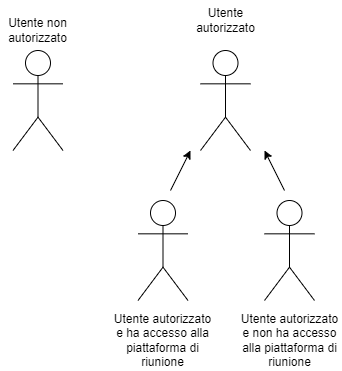
\includegraphics[scale=0.70]{images/Attori.png}
\end{center}
\newpage
\section{Casi d'Uso}
\subsection{UC1 - Autenticazione}
\begin{itemize}
    \item \textbf{Identificativo}: UC1
    \item \textbf{Nome}: Gestione autenticazione
    \item \textbf{Descrizione grafica}:
\end{itemize}

\begin{figure}[h]
    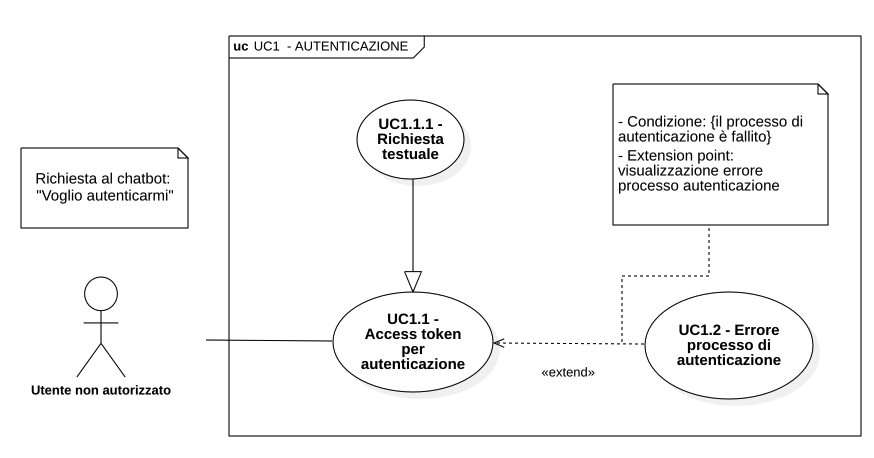
\includegraphics[scale=0.50]{images/UC1.png} 
    \caption{Descrizione grafica caso d'uso UC1}
\end{figure}

 \begin{itemize}
    \item \textbf{Attori}
 \begin{itemize} 
    \item \textit{Primari}: utente non autorizzato
    \item \textit{Secondari}: non presenti
 \end{itemize}
 \item \textbf{Precondizione}: l'utente vuole utilizzare i servizi messi a disposizione dal chatbot e dispone di un access token\textsubscript{G}.
 \item \textbf{Postcondizione}: l'utente si autentica al sistema e può utilizzare il servizio.
 \item \textbf{Scenario principale}: l'utente vuole effettuare il login al sistema, ha a disposizione un access token\textsubscript{G} che fornirà al chatbot per autenticarsi.
 \item \textbf{Scenario secondario:} se l'utente prova ad autenticarsi con un token\textsubscript{G} di accesso non valido viene visualizzato un messaggio di errore. (\textbf{UC1.2})
\end{itemize}
\newpage

\subsubsection{UC1.1 - Token di accesso autenticazione}
\begin{itemize}
    \item \textbf{Identificativo}: UC1.1
    \item \textbf{Nome}: token\textsubscript{G} di accesso autenticazione
    \item \textbf{Descrizione grafica}: (approfondita in UC1)
    \item \textbf{Attori}
 \begin{itemize} 
    \item \textit{Primari}: utente non autorizzato
    \item \textit{Secondari}: non presenti
 \end{itemize}
 \item \textbf{Precondizione}: l'utente ha a disposizione un token\textsubscript{G} di accesso.
 \item \textbf{Postcondizione}: l'utente fornisce il token\textsubscript{G} al chatbot.
 \item \textbf{Scenario principale}: l'utente fornisce il token\textsubscript{G} al chatbot in maniera testuale (UC1.1.1). Se il token\textsubscript{G} fornito è valido allora l'utente avrà effettuato il login correttamente e potrà usufruire dei servizi messi a disposizione. 
 \item \textbf{Scenario secondario}: se il token\textsubscript{G} non risultasse essere valido, verrà mostrato un messaggio di errore ad esso relativo (\textbf{UC1.2})
\end{itemize}

\paragraph{UC1.1.1 - Richiesta Testuale}
\begin{itemize}
   \item \textbf{Identificativo}: UC1.1.1
   \item \textbf{Nome}: Richiesta testuale
   \item \textbf{Descrizione grafica}: (approfondita in UC1)
   \item \textbf{Attori}:
   \begin{itemize} 
       \item \textit{Primari}: utente autorizzato
       \item \textit{Secondari}: non presenti
   \end{itemize}
       \item \textbf{Precondizione}: l'utente dispone del proprio token\textsubscript{G} necessario per effettuare l'accesso.
       \item \textbf{Postcondizione}: l'utente ha comunicato al chatbot il proprio access token, tramite input testuale. 
    \item \textbf{Scenario principale}: 
       \begin{itemize}
           \item L'utente fornisce un input testuale al chatbot contenente il proprio accesso token\textsubscript{G} 
       \end{itemize}
\end{itemize}

\subsubsection{UC1.2 - Token non valido}
\begin{itemize}
    \item \textbf{Identificativo}: UC1.2
    \item \textbf{Nome}: token\textsubscript{G} non valido
    \item \textbf{Descrizione grafica}: (approfondita in UC1)
    \item \textbf{Attori}
 \begin{itemize} 
    \item \textit{Primari}: utente non autorizzato 
    \item \textit{Secondari}: non presenti
 \end{itemize}
 \item \textbf{Precondizione}: l'utente ha a disposizione un token\textsubscript{G} non valido.
 \item \textbf{Postcondizione}: chatbot nega l'accesso ai servizi, viene comunicato l'errore all'utente e riproposto il sistema di login.
 \item \textbf{Scenario principale}: il token\textsubscript{G} inserito dall'utente risulta essere non valido per l'accesso, viene mostrato un messaggio di errore e il chatbot propone all'utente di rieffettuare la procedura di login.
\end{itemize}
\newpage

\subsection{UC2 - Visualizzazione Errore Interpretazione}


\subsection{UC3 - Tracciamento PRESENZE\textsubscript{G} in sede}
\begin{itemize}
    \item \textbf{Identificativo}: UC3
    \item \textbf{Nome}: Tracciamento PRESENZE\textsubscript{G} in sede
    \item \textbf{Descrione grafica}:
    \item \textbf{Attori}
 \begin{itemize} 
    \item \textit{Primari}: utente autorizzato
    \item \textit{Secondari}: non presenti
 \end{itemize}
 \item \textbf{Precondizione}: l'utente sta scambiando una serie di messaggi con il chatbot con lo scopo di eseguire una determinata azione
 \item \textbf{Postcondizione}: il chatbot non è stato in grado di comprendere la richiesta dell'utente restituendo un messaggio di errore.  
 \item \textbf{Scenario principale}: 
\end{itemize}

\subsection{UC4 - Apertura cancello}
\begin{itemize}
    \item \textbf{Identificativo}: UC4
    \item \textbf{Nome}: apertura cancello
    \item \textbf{Descrizione grafica}:
\end{itemize}

\begin{figure}[h]
   \centering
   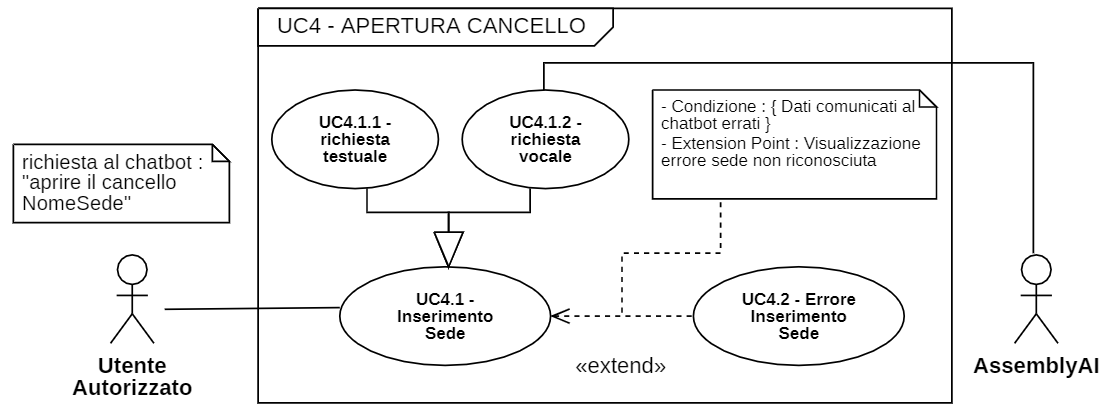
\includegraphics[scale=1.5]{images/UC4.png} 
   \caption{Descrizione grafica caso d'uso UC4}
\end{figure}


 \begin{itemize}
    \item \textbf{Attori}
 \begin{itemize} 
    \item \textit{Primari}: utente autorizzato
    \item \textit{Secondari}: non presenti
 \end{itemize}
 \item \textbf{Precondizione}: l'utente è autorizzato e si trova nell'interfaccia del chatbot.
 \item \textbf{Postcondizione}: il chatbot risponde alla richiesta dell'utente e invia la richiesta di apertura del cancello.
 \item \textbf{Scenario principale}: l'utente autorizzato richiede l'apertura del cancello, specificando la sede (UC4.1).
 \item \textbf{Estensioni}: 
 \begin{itemize} 
    \item il chatbot comunica all'utente che la sede specificata non è stata trovata (UC4.2).
 \end{itemize}
\end{itemize}
\newpage
\subsubsection{UC4.1 - Inserimento sede}
\begin{itemize}
    \item \textbf{Identificativo}: UC4.1
    \item \textbf{Nome}: inserimento sede
    \item \textbf{Descrizione grafica}: (approfondita in UC4)
    \item \textbf{Attori}
 \begin{itemize} 
    \item \textit{Primari}: utente autorizzato 
    \item \textit{Secondari}: non presenti
 \end{itemize}
 \item \textbf{Precondizione}: l'utente ha comunicato al chatbot la richiesta di apertura del cancello di una sede.
 \item \textbf{Postcondizione}: il chatbot inoltra la richiesta per la sede specificata.
 \item \textbf{Scenario principale}: il chatbot chiede all'utente di specificare di quale sede vuole aprire il cancello. L'utente comunica al chatbot la sede tramite messaggio testuale (UC4.1.1) o vocale (UC4.1.2).
\item \textbf{Estensioni}: 
 \begin{itemize} 
    \item il chatbot comunica all'utente che la sede specificata non è stata trovata (UC4.2).
 \end{itemize}
\end{itemize}

\paragraph{UC4.1.1 - Richiesta Testuale}
\begin{itemize}
   \item \textbf{Identificativo}: UC4.1.1
   \item \textbf{Nome}: Richiesta testuale
   \item \textbf{Descrizione grafica}: (approfondita in UC4)
   \item \textbf{Attori}:
   \begin{itemize} 
       \item \textit{Primari}: utente autorizzato
       \item \textit{Secondari}: non presenti
   \end{itemize}
       \item \textbf{Precondizione}: l'utente si è autenticato al sistema e ha richiesto di voler aprire il cancello di una sede. 
       \item \textbf{Postcondizione}: l'utente fornisce il nome della sede della quale voler aprire il cancello.
    \item \textbf{Scenario principale}: 
       \begin{itemize}
           \item L'utente ha effettuato l'accesso al sistema 
           \item L'utente fornisce tramite input testuale il nome della sede, di cui vuole aprire il cancelllo
       \end{itemize}
\end{itemize}

\paragraph{UC4.1.2 - Richiesta Vocale}
\begin{itemize}
   \item \textbf{Identificativo}: UC4.1.1
   \item \textbf{Nome}: Richiesta vocale
   \item \textbf{Descrizione grafica}: (approfondita in UC4)
   \item \textbf{Attori}:
   \begin{itemize} 
       \item \textit{Primari}: utente autorizzato
       \item \textit{Secondari}: non presenti
   \end{itemize}
       \item \textbf{Precondizione}: l'utente si è autenticato al sistema e ha richiesto di voler aprire il cancello di una sede. 
       \item \textbf{Postcondizione}: l'utente fornisce il nome della sede della quale voler aprire il cancello.
    \item \textbf{Scenario principale}: 
       \begin{itemize}
           \item L'utente ha effettuato l'accesso al sistema 
           \item L'utente fornisce tramite input vocale il nome della sede, di cui vuole aprire il cancelllo
       \end{itemize}
\end{itemize}

\subsubsection{UC4.2 - Errore inserimento sede}
\begin{itemize}
    \item \textbf{Identificativo}: UC4.5
    \item \textbf{Nome}: errore inserimento sede
    \item \textbf{Descrizione grafica}: (approfondita in UC4)
    \item \textbf{Attori}
 \begin{itemize} 
    \item \textit{Primari}: utente autorizzato 
    \item \textit{Secondari}: non presenti
 \end{itemize}
 \item \textbf{Precondizione}: l'utente ha comunicato al chatbot una sede non corretta.
 \item \textbf{Postcondizione}: il chatbot comunica all'utente che la sede inserita non è stata trovata.
 \item \textbf{Scenario principale}: il chatbot comunica all'utente che la sede inserita non è stata trovata e chiede di reinserirla.
\end{itemize}
\newpage

\subsection{UC5 - Apertura cancello}
\begin{itemize}
    \item \textbf{Identificativo}: UC5
    \item \textbf{Nome}: apertura cancello
    \item \textbf{Descrizione grafica}:
\end{itemize}

\begin{center}
    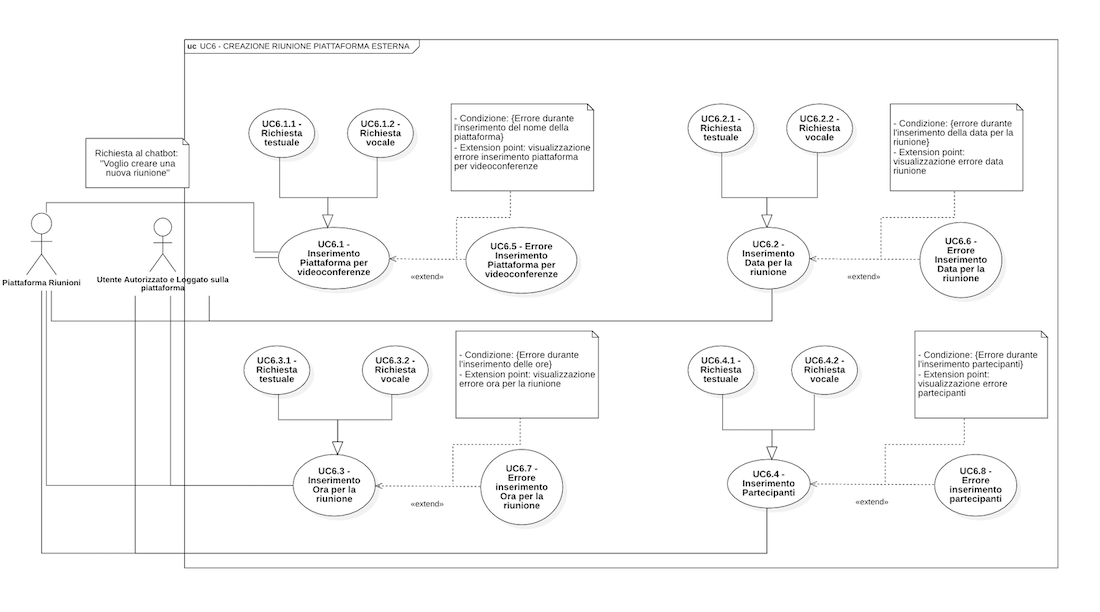
\includegraphics{images/UC5.png} 
\end{center} 

 \begin{itemize}
    \item \textbf{Attori}
 \begin{itemize} 
    \item \textit{Primari}: utente autorizzato
    \item \textit{Secondari}: non presenti
 \end{itemize}
 \item \textbf{Precondizione}: l'utente è autorizzato e si trova nell'interfaccia del chatbot.
 \item \textbf{Postcondizione}: il chatbot risponde alla richiesta dell'utente e invia la richiesta di apertura del cancello.
 \item \textbf{Scenario principale}: l'utente autorizzato richiede l'apertura del cancello, specificando la sede (UC5.1).
 \item \textbf{Estensioni}: 
 \begin{itemize} 
    \item il chatbot comunica all'utente che l'azione non è andata a buon fine (UC10).
    \item il chatbot comunica all'utente che non è stato in grado di interpretare il comando (UC2).
    \item il chatbot comunica all'utente che la sede specificata non è stata trovata (UC5.2).
 \end{itemize}
\end{itemize}
\newpage
\subsubsection{UC5.1 - Inserimento sede}
\begin{itemize}
    \item \textbf{Identificativo}: UC5.1
    \item \textbf{Nome}: inserimento sede
    \item \textbf{Descrizione grafica}: (approfondita in UC5)
    \item \textbf{Attori}
 \begin{itemize} 
    \item \textit{Primari}: utente autorizzato 
    \item \textit{Secondari}: non presenti
 \end{itemize}
 \item \textbf{Precondizione}: l'utente ha comunicato al chatbot la richiesta di apertura del cancello di una sede.
 \item \textbf{Postcondizione}: il chatbot inoltra la richiesta per la sede specificata.
 \item \textbf{Scenario principale}: il chatbot chiede all'utente di specificare di quale sede vuole aprire il cancello. L'utente comunica al chatbot la sede tramite messaggio testuale (UC5.1.1) o vocale (UC5.1.2).
\item \textbf{Estensioni}: 
 \begin{itemize} 
    \item il chatbot comunica all'utente che la sede specificata non è stata trovata (UC5.2).
 \end{itemize}
\end{itemize}
\subsubsection{UC5.2 - Errore inserimento sede}
\begin{itemize}
    \item \textbf{Identificativo}: UC5.5
    \item \textbf{Nome}: errore inserimento sede
    \item \textbf{Descrizione grafica}: (approfondita in UC5)
    \item \textbf{Attori}
 \begin{itemize} 
    \item \textit{Primari}: utente autorizzato 
    \item \textit{Secondari}: non presenti
 \end{itemize}
 \item \textbf{Precondizione}: l'utente ha comunicato al chatbot una sede non corretta.
 \item \textbf{Postcondizione}: il chatbot comunica all'utente che la sede inserita non è stata trovata.
 \item \textbf{Scenario principale}: il chatbot comunica all'utente che la sede inserita non è stata trovata e chiede di reinserirla.
\end{itemize}
\newpage

\subsection{UC6 - Ricerca documentale}
\begin{itemize}
    \item \textbf{Identificativo}: UC6
    \item \textbf{Nome}: ricerca documentale
    \item \textbf{Descrizione grafica}:
\end{itemize}

\begin{figure}[h]
   \centering
   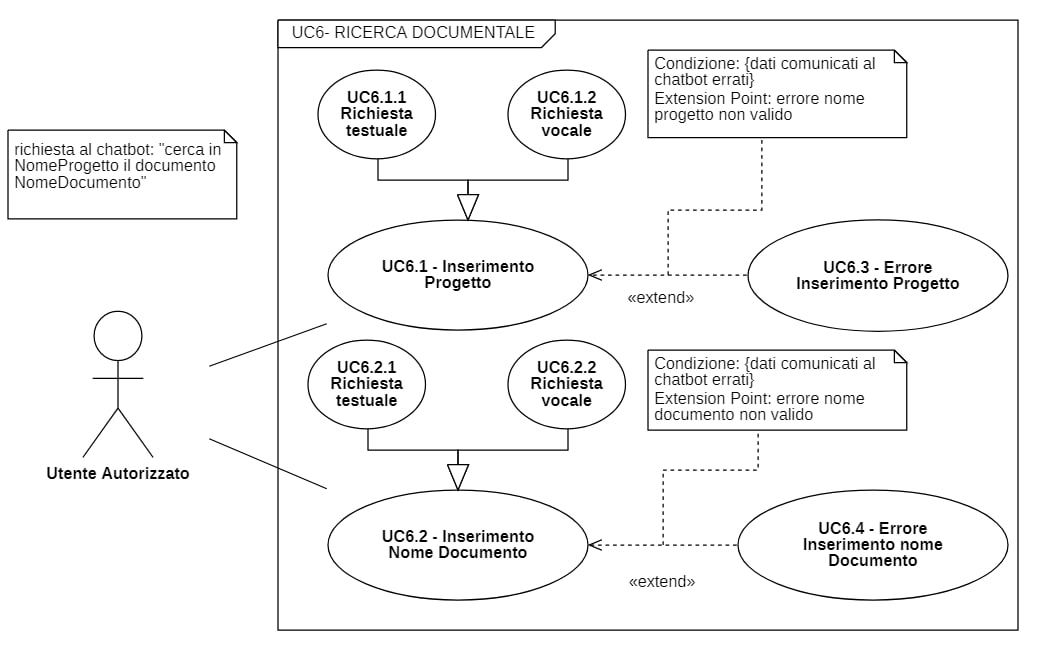
\includegraphics[scale=2]{images/UC6.png} 
   \caption{Descrizione grafica caso d'uso UC6}
\end{figure}

 \begin{itemize}
    \item \textbf{Attori}
 \begin{itemize} 
    \item \textit{Primari}: utente autorizzato
    \item \textit{Secondari}: non presenti
 \end{itemize}
 \item \textbf{Precondizione}: l'utente è autorizzato e si trova nell'interfaccia del chatbot.
 \item \textbf{Postcondizione}: il chatbot risponde alla richiesta dell'utente mostrando i documenti trovati.
 \item \textbf{Scenario principale}: l'utente autorizzato chiede al chatbot la ricerca di documenti, specificando il progetto al quale è associato (UC6.1) e il nome del documento (UC6.2).
 \item \textbf{Estensioni}: 
 \begin{itemize} 
    \item il chatbot comunica all'utente che l'inserimento del nome del progetto (UC6.3) o del nome del documento (UC6.4) non sono corretti.
 \end{itemize}
\end{itemize}
\newpage
\subsubsection{UC6.1 - Inserimento progetto}
\begin{itemize}
    \item \textbf{Identificativo}: UC6.1
    \item \textbf{Nome}: inserimento progetto
    \item \textbf{Descrizione grafica}: (approfondita in UC6)
    \item \textbf{Attori}
 \begin{itemize} 
    \item \textit{Primari}: utente autorizzato
    \item \textit{Secondari}: non presenti
 \end{itemize}
 \item \textbf{Precondizione}: l'utente ha richiesto al chatbot la ricerca di un documento.
 \item \textbf{Postcondizione}:  l'utente ha comunicato al chatbot il progetto nel quale ricercare i documenti.
 \item \textbf{Scenario principale}: il chatbot chiede all'utente di specificare il progetto nel quale ricercare i documenti. L'utente comunica al chatbot il progetto tramite messaggio testuale (UC6.1.1) o vocale (UC6.1.2).
 \item \textbf{Estensioni}: 
 \begin{itemize} 
    \item il chatbot comunica all'utente che il nome del progetto inserito non è corretto (UC6.3).
 \end{itemize}
\end{itemize}

\paragraph{UC6.1.1 - Richiesta Testuale}
\begin{itemize}
   \item \textbf{Identificativo}: UC6.1.1
   \item \textbf{Nome}: Richiesta testuale
   \item \textbf{Descrizione grafica}: (approfondita in UC6)
   \item \textbf{Attori}:
   \begin{itemize} 
       \item \textit{Primari}: utente autorizzato
       \item \textit{Secondari}: non presenti
   \end{itemize}
       \item \textbf{Precondizione}: l'utente si è autenticato al sistema e ha richiesto di voler cercare un documento all'interno di un progetto.
       \item \textbf{Postcondizione}: l'utente fornisce il nome del progetto in maniera testuale
    \item \textbf{Scenario principale}: 
       \begin{itemize}
           \item L'utente ha effettuato l'accesso al sistema 
           \item L'utente fornisce tramite input testuale il nome del progetto su cui fare la ricerca del documento
       \end{itemize}
\end{itemize}

\paragraph{UC6.1.2 - Richiesta Vocale}
\begin{itemize}
   \item \textbf{Identificativo}: UC6.1.2
   \item \textbf{Nome}: Richiesta vocale
   \item \textbf{Descrizione grafica}: (approfondita in UC6)
   \item \textbf{Attori}:
   \begin{itemize} 
       \item \textit{Primari}: utente autorizzato
       \item \textit{Secondari}: non presenti
   \end{itemize}
       \item \textbf{Precondizione}: l'utente si è autenticato al sistema e ha richiesto di voler cercare un documento all'interno di un progetto.
       \item \textbf{Postcondizione}: l'utente fornisce il nome del progetto in maniera vocale
    \item \textbf{Scenario principale}: 
       \begin{itemize}
           \item L'utente ha effettuato l'accesso al sistema 
           \item L'utente fornisce tramite input vocale il nome del progetto su cui fare la ricerca del documento
       \end{itemize}
\end{itemize}

\subsubsection{UC6.2 - Inserimento nome documento}
\begin{itemize}
    \item \textbf{Identificativo}: UC6.2
    \item \textbf{Nome}: inserimento nome documento
    \item \textbf{Descrizione grafica}: (approfondita in UC6)
    \item \textbf{Attori}
 \begin{itemize} 
    \item \textit{Primari}: utente autorizzato
    \item \textit{Secondari}: non presenti
 \end{itemize}
 \item \textbf{Precondizione}: l'utente ha richiesto al chatbot la ricerca di un documento.
 \item \textbf{Postcondizione}:  l'utente ha comunicato al chatbot il nome del documento da ricercare.
 \item \textbf{Scenario principale}: il chatbot chiede all'utente di specificare il nome del documento da ricercare. L'utente comunica al chatbot il nome del documento tramite messaggio testuale (UC6.1.1) o vocale (UC6.1.2).
 \item \textbf{Estensioni}: 
\begin{itemize} 
    \item il chatbot comunica all'utente che il nome del documento inserito non è corretto (UC6.4).
 \end{itemize}
\end{itemize}

\paragraph{UC6.2.1 - Richiesta Testuale}
\begin{itemize}
   \item \textbf{Identificativo}: UC6.2.1
   \item \textbf{Nome}: Richiesta testuale
   \item \textbf{Descrizione grafica}: (approfondita in UC6)
   \item \textbf{Attori}:
   \begin{itemize} 
       \item \textit{Primari}: utente autorizzato
       \item \textit{Secondari}: non presenti
   \end{itemize}
       \item \textbf{Precondizione}: l'utente si è autenticato al sistema e ha richiesto di voler cercare un documento all'interno di un progetto.
       \item \textbf{Postcondizione}: l'utente fornisce il nome del documento in maniera testuale
    \item \textbf{Scenario principale}: 
       \begin{itemize}
           \item L'utente ha effettuato l'accesso al sistema 
           \item L'utente fornisce tramite input testuale il nome del documento da ricercare
       \end{itemize}
\end{itemize}

\paragraph{UC6.2.2 - Richiesta Vocale}
\begin{itemize}
   \item \textbf{Identificativo}: UC6.2.2
   \item \textbf{Nome}: Richiesta vocale
   \item \textbf{Descrizione grafica}: (approfondita in UC6)
   \item \textbf{Attori}:
   \begin{itemize} 
       \item \textit{Primari}: utente autorizzato
       \item \textit{Secondari}: non presenti
   \end{itemize}
       \item \textbf{Precondizione}: l'utente si è autenticato al sistema e ha richiesto di voler cercare un documento all'interno di un progetto.
       \item \textbf{Postcondizione}: l'utente fornisce il nome del documento in maniera vocale
    \item \textbf{Scenario principale}: 
       \begin{itemize}
           \item L'utente ha effettuato l'accesso al sistema 
           \item L'utente fornisce tramite input vocale il nome del documento da ricercare
       \end{itemize}
\end{itemize}

\subsubsection{UC6.3 - Errore inserimento nome progetto}
\begin{itemize}
    \item \textbf{Identificativo}: UC6.3
    \item \textbf{Nome}: errore inserimento nome progetto
    \item \textbf{Descrizione grafica}: (approfondita in UC6)
    \item \textbf{Attori}
 \begin{itemize} 
    \item \textit{Primari}: utente autorizzato
    \item \textit{Secondari}: non presenti
 \end{itemize}
 \item \textbf{Precondizione}: l'utente ha inserito un nome di progetto non valido.
 \item \textbf{Postcondizione}:  il chatbot comunica all'utente che il nome di progetto specificato non è corretto.
 \item \textbf{Scenario principale}: il chatbot comunica all'utente l'errore nell'inserimento del nome di progetto e chiede di reinserirlo.
\end{itemize}
\subsubsection{UC6.4 - Errore inserimento nome documento}
\begin{itemize}
    \item \textbf{Identificativo}: UC6.4
    \item \textbf{Nome}: errore inserimento nome documento
    \item \textbf{Descrizione grafica}: (approfondita in UC6)
    \item \textbf{Attori}
 \begin{itemize} 
    \item \textit{Primari}: utente autorizzato
    \item \textit{Secondari}: non presenti
 \end{itemize}
 \item \textbf{Precondizione}: l'utente ha inserito un nome documento non valido.
 \item \textbf{Postcondizione}:  il chatbot comunica all'utente che il nome del documento specificato non è corretto.
 \item \textbf{Scenario principale}: il chatbot comunica all'utente l'errore nell'inserimento del nome del documento e chiede di reinserirlo.
\end{itemize}
\newpage

\subsection{UC7 - Inserimento \glossario{ticket}}
\begin{itemize}
	\item \textbf{Identificativo}: UC7
	\item \textbf{Nome}: Inserimento \glossario{ticket}
	\item\textbf{Descrizione Grafica}: 
	

	\begin{figure}[h]
        \centering
        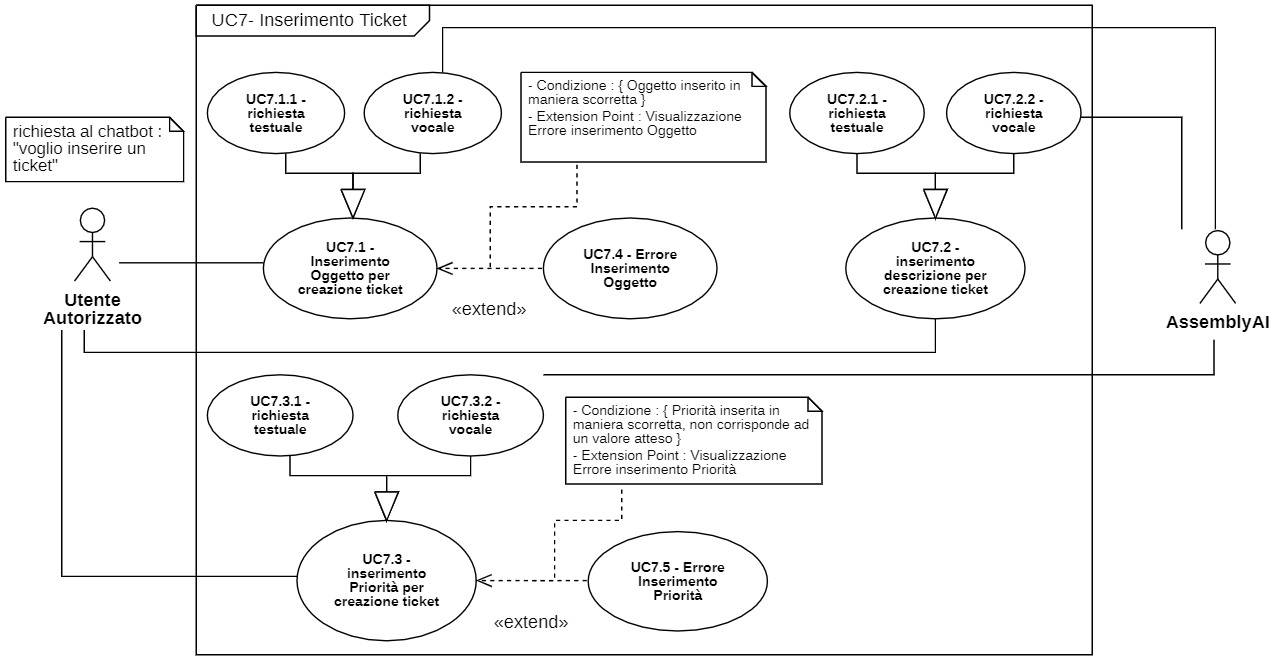
\includegraphics[scale=0.80]{images/UC7.png} 
        \caption{Descrizione grafica caso d'uso UC7}
    \end{figure}

	\item \textbf{Attori}
	\begin{itemize} 
		\item \textit{Primari}: Utente autorizzato
		\item \textit{Secondari}: Non presenti 
	\end{itemize}
	\item \textbf{Descrizione}: L'utente vuole creare un nuovo \glossario{ticket}. Dopo aver ricevuto la richiesta, il chatbot richiede le informazione necessarie al fine di creare un ticket. Il chatbot potrà dover chiedere ulteriori informazioni mancanti o, in caso di errore, comunicare all'utente l'impossibilità di creazione del \glossario{ticket}.
	\item \textbf{Precondizione}: L'utente ha effettuato il login e si trova nella chat.
	\item \textbf{Postcondizione}: \glossario{Ticket} creato con successo.
	\item \textbf{Scenario principale}: \begin{enumerate}
		\item Utente inserisce un messaggio del tipo "Voglio creare un nuovo Ticket";
		\item Chatbot chiede all'utente l'oggeto del \glossario{ticket}; (UC7.1)
    \item Chatbot chiede all'utente la descrizione; (UC7.2)
		\item Chatbot chiede all'utente la priorità. (UC7.3)
	\end{enumerate}
\end{itemize}


\subsubsection{UC7.1 - Inserimento Oggetto per creazione \glossario{ticket}}
\begin{itemize}
	\item \textbf{Identificativo}: UC7.1
	\item \textbf{Nome}: Inserimento Oggetto per creazione \glossario{ticket} 
	\item \textbf{Attori}
	\begin{itemize} 
		\item \textit{Primari}: Utente autorizzato
		\item \textit{Secondari}: Non presenti
	\end{itemize}
	\item \textbf{Descrizione}: L'utente sta eseguendo il procedimento di creazione di un nuovo \glossario{ticket}. Il chatbot richiede all'utente di inserire un Oggetto. 
	\item \textbf{Precondizione}: L'utente ha iniziato la procedura di creazione di un \glossario{ticket}.
	\item \textbf{Postcondizione}: L'utente ha comunicato al chatbot l'oggetto del nuovo ticket.
	\item \textbf{Scenario principale}: \begin{enumerate}
		\item Chatbot interagisce con l'utente: "Indicare l'oggetto del ticket";
		\item Utente fornisce l'oggetto per la creazione del ticket tramite testo (UC7.1.1) o input vocale (UC7.1.2). 
	\end{enumerate}
	\item \textbf{Estensione}: Utente non ha inserito l'oggetto in maniera idonea per il chatbot. (UC7.4)		
\end{itemize}

\paragraph{UC7.1.1 - Richiesta Testuale}
\begin{itemize}
   \item \textbf{Identificativo}: UC7.1.1
   \item \textbf{Nome}: Richiesta testuale
   \item \textbf{Descrizione grafica}: (approfondita in UC7)
   \item \textbf{Attori}:
   \begin{itemize} 
       \item \textit{Primari}: utente autorizzato
       \item \textit{Secondari}: non presenti
   \end{itemize}
       \item \textbf{Precondizione}: L'utente sta creando un ticket e gli è richiesto l'inserimento di un oggetto.
       \item \textbf{Postcondizione}: L'utente comunica un oggetto e procede con la creazione del ticket. 
    \item \textbf{Scenario principale}: 
       \begin{itemize}
           \item Il chatbot richiede l'inserimento di un oggetto;
           \item l'utente inserisce testualmente un oggetto.
       \end{itemize}
\end{itemize}

\paragraph{UC7.1.2 - Richiesta Vocale}
\begin{itemize}
   \item \textbf{Identificativo}: UC7.1.2
   \item \textbf{Nome}: Richiesta Vocale
   \item \textbf{Descrizione grafica}: (approfondita in UC7)
   \item \textbf{Attori}:
   \begin{itemize} 
       \item \textit{Primari}: utente autorizzato
       \item \textit{Secondari}: non presenti
   \end{itemize}
       \item \textbf{Precondizione}: L'utente sta creando un ticket e gli è richiesto l'inserimento di un oggetto.
       \item \textbf{Postcondizione}: L'utente comunica un oggetto e procede con la creazione del ticket. 
    \item \textbf{Scenario principale}: 
       \begin{itemize}  
        \item Il chatbot richiede l'inserimento di un oggetto;
        \item l'utente inserisce vocalmente un oggetto.
       \end{itemize}
\end{itemize}


\subsubsection{UC7.2 - Inserimento descrizione per creazione \glossario{ticket}}
\begin{itemize}
	\item \textbf{Identificativo}: UC7.2
	\item \textbf{Nome}: Inserimento descrizione per creazione \glossario{ticket} 
	\item \textbf{Attori}
	\begin{itemize} 
		\item \textit{Primari}: Utente autorizzato
		\item \textit{Secondari}: Non presenti
	\end{itemize}
	\item \textbf{Descrizione}:  Utente sta eseguendo il procedimento di creazione di un nuovo \glossario{ticket}. Il chatbot richiede all'utente di inserire una descrizione. 
	\item \textbf{Precondizione}: Utente ha comunicato al chatbot l'oggetto del nuovo ticket.
	\item \textbf{Postcondizione}: Utente ha comunicato al chatbot la descrizione del nuovo ticket.
	\item \textbf{Scenario principale}: \begin{enumerate}
		\item Chatbot interagisce con l'utente: "Indicare la descrizione del ticket";
		\item Utente fornisce la descrizione per la creazione del ticket tramite testo (UC7.2.1) o input vocale (UC7.2.2).
	\end{enumerate}
	\end{itemize}

  \paragraph{UC7.2.1 - Richiesta Testuale}
  \begin{itemize}
     \item \textbf{Identificativo}: UC7.2.1
     \item \textbf{Nome}: Richiesta testuale
     \item \textbf{Descrizione grafica}: (approfondita in UC7)
     \item \textbf{Attori}:
     \begin{itemize} 
         \item \textit{Primari}: utente autorizzato
         \item \textit{Secondari}: non presenti
     \end{itemize}
         \item \textbf{Precondizione}: L'utente sta creando un ticket, ha inserito un oggetto e gli è richiesto l'inserimento di una descrizione.
         \item \textbf{Postcondizione}: L'utente comunica una descrizione e procede con la creazione del ticket. 
      \item \textbf{Scenario principale}: 
         \begin{itemize}
             \item Il chatbot richiede l'inserimento di una descrizione;
             \item l'utente inserisce testualmente una descrizione.
         \end{itemize}
  \end{itemize}
  
  \paragraph{UC7.2.2 - Richiesta Vocale}
  \begin{itemize}
     \item \textbf{Identificativo}: UC7.2.2
     \item \textbf{Nome}: Richiesta testuale
     \item \textbf{Descrizione grafica}: (approfondita in UC7)
     \item \textbf{Attori}:
     \begin{itemize} 
         \item \textit{Primari}: utente autorizzato
         \item \textit{Secondari}: non presenti
     \end{itemize}
         \item \textbf{Precondizione}: L'utente sta creando un ticket, ha inserito un oggetto e gli è richiesto l'inserimento di una descrizione.
         \item \textbf{Postcondizione}: L'utente comunica una descrizione e procede con la creazione del ticket. 
      \item \textbf{Scenario principale}: 
         \begin{itemize}  
          \item Il chatbot richiede l'inserimento di una descrizione;
          \item l'utente inserisce vocalmente una descrizione.
         \end{itemize}
  \end{itemize}


  \subsubsection{UC7.3 - Inserimento priorità per creazione \glossario{ticket}}
\begin{itemize}
	\item \textbf{Identificativo}: UC7.3
	\item \textbf{Nome}: Inserimento priorità per creazione \glossario{ticket}
	\item \textbf{Attori}
	\begin{itemize} 
		\item \textit{Primari}: Utente autorizzato
		\item \textit{Secondari}: Non presenti
	\end{itemize}
	\item \textbf{Descrizione}: L'utente sta eseguendo il procedimento di creazione di un nuovo \glossario{ticket}. Il chatbot richiede all'utente di assegnare una priorità.
	\item \textbf{Precondizione}: l'utente ha comunicato al chatbot la priorità del nuovo ticket.
	\item \textbf{Postcondizione}: l'utente ha comunicato al chatbot la priorità del nuovo ticket.
	\item \textbf{Scenario principale}: \begin{enumerate}
		\item Chatbot interagisce con l'utente: "Assegnare una priorità al ticket";
		\item Utente assegna una priorità al ticket tramite testo (UC7.4.1) o input vocale (UC7.4.2).
	\end{enumerate}
	\item \textbf{Estensione}: L'utente non ha inserito la priorità in maniera idonea per il chatbot. (UC7.5)
\end{itemize}

\paragraph{UC7.3.1 - Richiesta Testuale}
\begin{itemize}
   \item \textbf{Identificativo}: UC7.3.1
   \item \textbf{Nome}: Richiesta testuale
   \item \textbf{Descrizione grafica}: (approfondita in UC7)
   \item \textbf{Attori}:
   \begin{itemize} 
       \item \textit{Primari}: utente autorizzato
       \item \textit{Secondari}: non presenti
   \end{itemize}
       \item \textbf{Precondizione}: L'utente sta creando un ticket e gli è richiesto l'inserimento di una priorità.
       \item \textbf{Postcondizione}: L'utente comunica una priorità e viene creato il ticket. 
    \item \textbf{Scenario principale}: 
       \begin{itemize}
           \item Il chatbot richiede l'inserimento di una priorità;
           \item l'utente inserisce testualmente una priorità.
       \end{itemize}
\end{itemize}

\paragraph{UC7.3.2 - Richiesta Vocale}
\begin{itemize}
   \item \textbf{Identificativo}: UC7.3.2
   \item \textbf{Nome}: Richiesta Vocale
   \item \textbf{Descrizione grafica}: (approfondita in UC7)
   \item \textbf{Attori}:
   \begin{itemize} 
       \item \textit{Primari}: utente autorizzato
       \item \textit{Secondari}: non presenti
   \end{itemize}
   \item \textbf{Precondizione}: L'utente sta creando un ticket e gli è richiesto l'inserimento di una priorità.
   \item \textbf{Postcondizione}: L'utente comunica una priorità e viene creato il ticket. 
    \item \textbf{Scenario principale}: 
       \begin{itemize}  
        \item Il chatbot richiede l'inserimento di una priorità;
        \item l'utente inserisce vocalmente una priorità.
       \end{itemize}
\end{itemize}

\subsubsection{UC7.4 - Visualizzazione errore inserimento oggetto}
\begin{itemize}
	\item \textbf{Identificativo}: UC7.4
	\item \textbf{Nome}: Visualizzazione errore inserimento oggetto 
	\item \textbf{Attori}
	\begin{itemize} 
		\item \textit{Primari}: Utente autorizzato
		\item \textit{Secondari}: Non presenti
	\end{itemize}
	\item \textbf{Descrizione}: È avvenuto un errore nell'inserimento dell'oggetto. Il chatbot mostra l'errore all'utente.
	\item \textbf{Precondizione}: L'utente sta eseguendo l'operazione di inserimento di un nuovo ticket. L'oggetto risulta essere inserito in un formato non valido. 
	\item \textbf{Postcondizione}: Il chatbot mostra all'utente che l'oggetto non è stato inserito in maniera idonea per il chatbot.
	\item \textbf{Scenario principale}: \begin{enumerate}
		\item Chatbot mostra all'utente che è avvenuto un errore tramite chat: "Oggetto inserito in maniera non idonea".
		\end{enumerate}
\end{itemize}


\subsubsection{UC7.5 - Visualizzazione errore inserimento priorità}
\begin{itemize}
	\item \textbf{Identificativo}: UC7.5
	\item \textbf{Nome}:  Visualizzazione errore inserimento priorità
	\item \textbf{Attori}
	\begin{itemize} 
		\item \textit{Primari}: Utente autorizzato
		\item \textit{Secondari}: Non presenti
	\end{itemize}
	\item \textbf{Descrizione}: È avvenuto un errore nell'inserimento della priorità. Il chatbot mostra l'errore all'utente.
	\item \textbf{Precondizione}: L'utente sta eseguendo l'operazione di inserimento di un nuovo ticket. La priorità risulta essere inserita in un formato non valido. 
	\item \textbf{Postcondizione}: Il chatbot mostra all'utente che la priorità non è stata inserita in maniera idonea per il chatbot o non assume uno dei valori fissi che il chatbot si aspetta.
	\item \textbf{Scenario principale}: \begin{enumerate}
		\item Chatbot mostra all'utente che è avvenuto un errore tramite chat: "Priorità inserita in maniera non idonea".
	\end{enumerate}
\end{itemize}
\newpage

\subsection{UC8 - Annullamento Operazione }
\begin{itemize}
	\item \textbf{Identificativo}: UC8
	\item \textbf{Nome}: Annullamento Operazione
  \item \textbf{Descrizione grafica}:

\begin{figure}[h]
    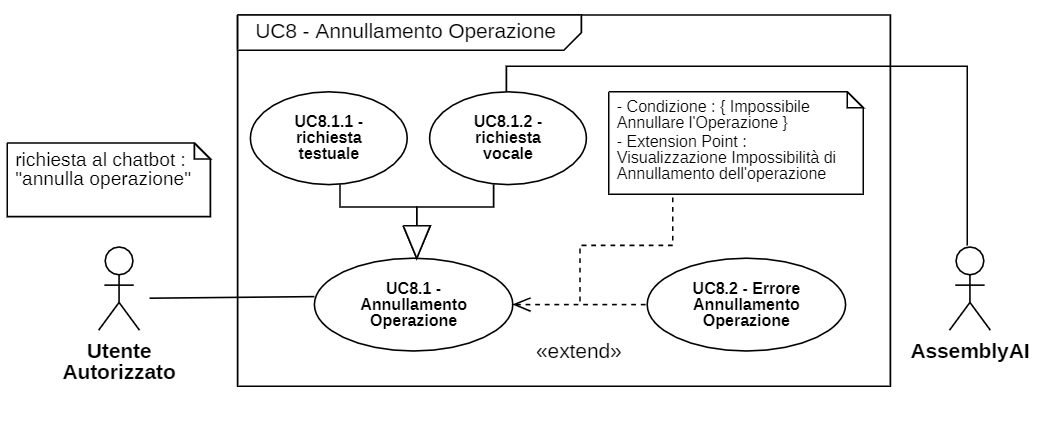
\includegraphics[scale=1.20]{images/UC8.png} 
    \caption{Descrizione grafica caso d'uso UC8}
\end{figure}

	\item \textbf{Attori}
	\begin{itemize} 
		\item \textit{Primari}: Utente autorizzato
		\item \textit{Secondari}: Non presenti
	\end{itemize}
	\item \textbf{Descrizione}: L'utente vuole cancellare esecuzione di un'operazione precedentemente richiesta.
	\item \textbf{Precondizione}: L'utente ha richiesto un'operazione.
	\item \textbf{Postcondizione}: Operazione non viene eseguita.
	\item \textbf{Scenario principale}: \begin{enumerate}
		\item Utente comunica al chatbot: "Annulla operazione";
		\item Chatbot comunica: "Operazione annullata con successo".
	\end{enumerate}
  \item \textbf{Estensione}: L'operazione di annullamento non può essere eseguita. (UC8.2)
\end{itemize}

\paragraph{UC8.1.1 - Richiesta Testuale}
\begin{itemize}
   \item \textbf{Identificativo}: UC8.1.1
   \item \textbf{Nome}: Richiesta testuale
   \item \textbf{Descrizione grafica}: (approfondita in UC8)
   \item \textbf{Attori}:
   \begin{itemize} 
       \item \textit{Primari}: utente autorizzato
       \item \textit{Secondari}: non presenti
   \end{itemize}
       \item \textbf{Precondizione}: L'utente ha richiesto un'operazione.
       \item \textbf{Postcondizione}: Operazione non viene eseguita. 
    \item \textbf{Scenario principale}: 
       \begin{itemize}
        \item Utente scrive al chatbot: "Annulla operazione";
        \item Chatbot risponde: "Operazione annullata con successo".
       \end{itemize}
\end{itemize}

\paragraph{UC8.1.2 - Richiesta Vocale}
\begin{itemize}
   \item \textbf{Identificativo}: UC8.1.2
   \item \textbf{Nome}: Richiesta testuale
   \item \textbf{Descrizione grafica}: (approfondita in UC1)
   \item \textbf{Attori}:
   \begin{itemize} 
       \item \textit{Primari}: utente autorizzato
       \item \textit{Secondari}: non presenti
   \end{itemize}
       \item \textbf{Precondizione}: L'utente ha richiesto un'operazione.
       \item \textbf{Postcondizione}: Operazione non viene eseguita. 
    \item \textbf{Scenario principale}: 
       \begin{itemize}
        \item Utente comunica vocalmente al chatbot: "Annulla operazione";
        \item Chatbot comunica: "Operazione annullata con successo".
       \end{itemize}
\end{itemize}

\subsubsection{UC8.2 - Errore Annullamento Operazione}
\begin{itemize}
	\item \textbf{Identificativo}: UC8.2
	\item \textbf{Nome}: Errore Annullamento Operazione 
	\item \textbf{Attori}
	\begin{itemize} 
		\item \textit{Primari}: Utente autorizzato
		\item \textit{Secondari}: Non presenti
	\end{itemize}
	\item \textbf{Descrizione}: L'utente vuole annullare un'operazione.
	\item \textbf{Precondizione}: L'utente richiede di annullare un'operazione.
	\item \textbf{Postcondizione}: Viene visualizzato un errore di impossibilità di annullare l'operazione.
	\item \textbf{Scenario principale}: Utente comunica la volontà di annullare un'operazione ma questa viene negata.
\end{itemize}

\subsection{UC9 - Verifica dello stato di \glossario{Check-in}/Check-out}
\begin{itemize}
	\item \textbf{Identificativo}: UC9
	\item \textbf{Nome}: Verifica dello stato di \glossario{Check-in}/Check-out
	\item\textbf{Descrizione Grafica}: 
	
	\begin{figure}[h]
		\centering
		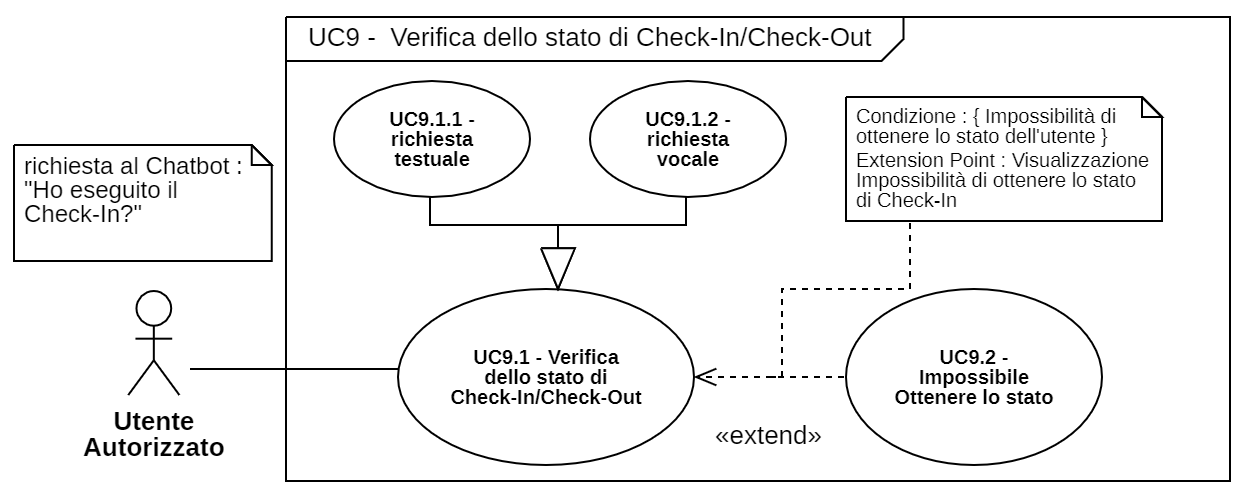
\includegraphics[scale=0.60]{images/UC9.png} 
		\caption{Descrizione grafica caso d'uso UC9}
	 \end{figure}

	\item \textbf{Attori}
	\begin{itemize} 
		\item \textit{Primari}: Utente autorizzato
		\item \textit{Secondari}: Non presenti
	\end{itemize}
	\item \textbf{Descrizione}: L'utente richiede conferma sull'attuale stato di \glossario{Check-in}/Check-out.
	\item \textbf{Precondizione}: L'utente ha effettuato il login e si trova nella chat.
	\item \textbf{Postcondizione}: Chatbot restituisce l'attuale stato di Check-in/Check-out.
	\item \textbf{Scenario principale}:  \begin{enumerate}
		\item Utente invia un messaggio del tipo : "Ho eseguito il check-in?";
		\item Chatbot risponde restituendo i Check-in/Check-out effettuati nella stessa data.
	\end{enumerate}
\end{itemize}

\subsubsection{UC9.1 Verifica dello stato di \glossario{Check-in}/Check-out}
\begin{itemize}
	\item \textbf{Identificativo}: UC9.1
	\item \textbf{Nome}: Verifica dello stato di \glossario{Check-in}/Check-out
	\item \textbf{Descrizione Grafica}: (Approfondita in UC9)
	\item \textbf{Attori}
	\begin{itemize}
		\item \textit{Primari}: Utente autorizzato
		\item \textit{Secondari}: Non presenti
	\end{itemize}
	\item \textbf{Descrizione}: L'utente richiede al chatbot di visualizzare il proprio stato di \glossario{check-in}/check-out.
	\item \textbf{Precondizione}: L'utente ha richiesto al chatbot di visualizzare il proprio stato.
	\item \textbf{Postcondizione}: Il chatbot comunica all'utente il suo stato.
	\item \textbf{Scenario principale}: Dopo che l'utente ha inviato la richiesta il chatbot visualizza lo stato di \glossario{check-in}/check-out.
\end{itemize}

\paragraph{UC9.1.1 Richiesta testuale}
\begin{itemize}
	\item \textbf{Identificativo}: UC9.1.1
	\item \textbf{Nome}: Richiesta testuale
	\item \textbf{Descrizione Grafica}: (Approfondita in UC9)
	\item \textbf{Attori}
	\begin{itemize}
		\item \textit{Primari}: Utente autorizzato
		\item \textit{Secondari}: Non presenti
	\end{itemize}
	\item \textbf{Descrizione}: L'utente effettua la richiesta tramite input testuale.
	\item \textbf{Precondizione}: L'utente vuole effettuare l'operazione.
	\item \textbf{Postcondizione}: L'utente comunica tramite formato testuale la richiesta al chatbot.
	\item \textbf{Scenario principale}: 
	\begin{enumerate}
		\item L'utente vuole richiedere la verifica dello stato di \glossario{Check-in}/Check-out;
		\item L'utente inserisce testualmente la richiesta.
	\end{enumerate}
\end{itemize}

\paragraph{UC9.1.2 Richiesta vocale}
\begin{itemize}
	\item \textbf{Identificativo}: UC9.1.2
	\item \textbf{Nome}: Richiesta vocale
	\item \textbf{Descrizione Grafica}: (Approfondita in UC9)
	\item \textbf{Attori}
	\begin{itemize}
		\item \textit{Primari}: Utente autorizzato
		\item \textit{Secondari}: Non presenti
	\end{itemize}
	\item \textbf{Descrizione}: L'utente effettua la richiesta tramite input vocale.
	\item \textbf{Precondizione}: L'utente vuole effettuare l'operazione.
	\item \textbf{Postcondizione}: L'utente comunica tramite formato vocale la richiesta al chatbot.
	\item \textbf{Scenario principale}: 
	\begin{enumerate}
		\item L'utente vuole richiedere la verifica dello stato di \glossario{Check-in}/Check-out;
		\item L'utente inserisce tramite input vocale la richiesta.
	\end{enumerate}
\end{itemize}

\subsubsection{UC9.2 Impossibile ottenere lo stato}
\begin{itemize}
	\item \textbf{Identificativo}: UC9.2
	\item \textbf{Nome}: Impossibile ottenere lo stato
	\item \textbf{Descrizione Grafica}: (Approfondita in UC9)
	\item \textbf{Attori}
	\begin{itemize}
		\item \textit{Primari}: Utente autorizzato
		\item \textit{Secondari}: Non presenti
	\end{itemize}
	\item \textbf{Descrizione}: L'utente richiede al chatbot di visualizzare il proprio stato di \glossario{check-in}/check-out ma viene visualizzato un messaggio d'errore.
	\item \textbf{Precondizione}: L'utente ha richiesto al chatbot di visualizzare il proprio stato.
	\item \textbf{Postcondizione}: Il chatbot comunica all'utente l'impossibilità di visualizzare lo stato.
	\item \textbf{Scenario principale}: L'utente richiede il proprio stato ma gli viene negato e visualizza un messaggio d'errore.
\end{itemize}
\newpage

\subsection{UC10 - Visualizzazione errore impossibile completare l'azione}


\subsection{UC11 - Annullamento Operazione }
\begin{itemize}
	\item \textbf{Identificativo}: UC11
	\item \textbf{Nome}: Annullamento Operazione
  \item \textbf{Descrizione grafica}:
\end{itemize}

\begin{figure}[h]
    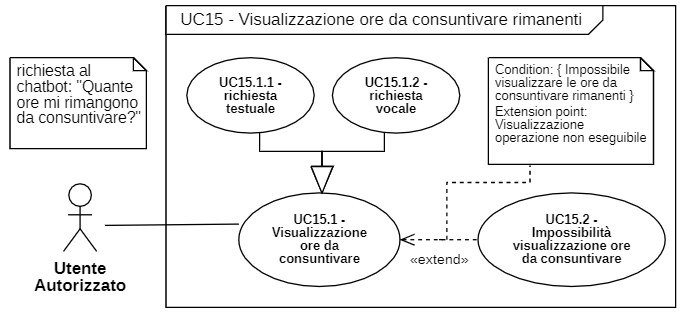
\includegraphics[scale=1.20]{images/UC11.png} 
    \caption{Descrizione grafica caso d'uso UC11}
\end{figure}
\begin{itemize}
	\item \textbf{Attori}
	\begin{itemize} 
		\item \textit{Primari}: Utente autorizzato
		\item \textit{Secondari}: Non presenti
	\end{itemize}
	\item \textbf{Descrizione}: L'utente vuole cancellare esecuzione di un'operazione precedentemente richiesta.
	\item \textbf{Precondizione}: L'utente ha richiesto un'operazione.
	\item \textbf{Postcondizione}: Operazione non viene eseguita.
	\item \textbf{Scenario principale}: \begin{enumerate}
		\item Utente comunica al chatbot: "Annulla operazione";
		\item Chatbot comunica: "Operazione annullata con successo".
	\end{enumerate}
  \item \textbf{Estensione}: L'operazione di annullamento non può essere eseguita. (UC11.2)
\end{itemize}

\paragraph{UC11.1.1 - Richiesta Testuale}
\begin{itemize}
   \item \textbf{Identificativo}: UC11.1.1
   \item \textbf{Nome}: Richiesta testuale
   \item \textbf{Descrizione grafica}: (approfondita in UC11)
   \item \textbf{Attori}:
   \begin{itemize} 
       \item \textit{Primari}: utente autorizzato
       \item \textit{Secondari}: non presenti
   \end{itemize}
       \item \textbf{Precondizione}: L'utente ha richiesto un'operazione.
       \item \textbf{Postcondizione}: Operazione non viene eseguita. 
    \item \textbf{Scenario principale}: 
       \begin{itemize}
        \item Utente scrive al chatbot: "Annulla operazione";
        \item Chatbot risponde: "Operazione annullata con successo".
       \end{itemize}
\end{itemize}

\paragraph{UC11.1.2 - Richiesta Vocale}
\begin{itemize}
   \item \textbf{Identificativo}: UC11.1.2
   \item \textbf{Nome}: Richiesta testuale
   \item \textbf{Descrizione grafica}: (approfondita in UC1)
   \item \textbf{Attori}:
   \begin{itemize} 
       \item \textit{Primari}: utente autorizzato
       \item \textit{Secondari}: non presenti
   \end{itemize}
       \item \textbf{Precondizione}: L'utente ha richiesto un'operazione.
       \item \textbf{Postcondizione}: Operazione non viene eseguita. 
    \item \textbf{Scenario principale}: 
       \begin{itemize}
        \item Utente comunica vocalmente al chatbot: "Annulla operazione";
        \item Chatbot comunica: "Operazione annullata con successo".
       \end{itemize}
\end{itemize}

\subsubsection{UC11.2 - Errore Annullamento Operazione}
\begin{itemize}
	\item \textbf{Identificativo}: UC11.2
	\item \textbf{Nome}: Errore Annullamento Operazione 
	\item \textbf{Attori}
	\begin{itemize} 
		\item \textit{Primari}: Utente autorizzato
		\item \textit{Secondari}: Non presenti
	\end{itemize}
	\item \textbf{Descrizione}: L'utente vuole annullare un'operazione.
	\item \textbf{Precondizione}: L'utente richiede di annullare un'operazione.
	\item \textbf{Postcondizione}: Viene visualizzato un errore di impossibilità di annullare l'operazione.
	\item \textbf{Scenario principale}: Utente comunica la volontà di annullare un'operazione ma questa viene negata.
\end{itemize}

\subsection{UC12 - (teoricamente da cancellare) Visualizzazione elenco documenti Trovati }
\begin{itemize}
	\item \textbf{Identificativo}: UC12
	\item \textbf{Nome}: Visualizzazione elenco documenti Trovati
	\item \textbf{Attori}
	\begin{itemize} 
		\item \textit{Primari}: Utente autorizzato
		\item \textit{Secondari}: Nessuno
	\end{itemize}
	\item \textbf{Descrizione}: L'utente viene informato della ricerca dei documenti trovati.
	\item \textbf{Precondizione}: L'utente ha effettuato la ricerca con successo.
	\item \textbf{Postcondizione}: Il chatbot invia all'utente l'elenco dei documenti.
	\item \textbf{Scenario principale}: \begin{enumerate}
		\item Chatbot comunica: "Ho trovato questi documenti ..." seguito dall'elenco dei documenti trovati.
	\end{enumerate}
\end{itemize}

\subsection{UC13 - Visualizzazione Riunioni Giornaliere }
\begin{itemize}
	\item \textbf{Identificativo}: UC13
	\item \textbf{Nome}: Visualizzazione Riunioni Giornaliere
	\item\textbf{Descrizione Grafica}: 
	\begin{center}
		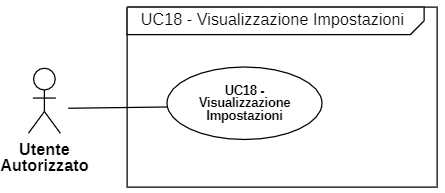
\includegraphics[scale=0.65]{images/UC13.png} 
	\end{center}

	\item \textbf{Attori}
	\begin{itemize} 
		\item \textit{Primari}: Utente autorizzato e autenticato nella \glossario{piattaforma riunioni}
		\item \textit{Secondari}: Non presenti
	\end{itemize}
	\item \textbf{Descrizione}: L'utente richiede di visualizzare le Riunioni del giorno.
	\item \textbf{Precondizione}: L'utente ha effettuato il login sia sull'app che sulla piattaforma esterna, e si trova nella chat.
	\item \textbf{Postcondizione}: Il chatbot restituisce la lista delle riunioni del giorno, con eventuali informazioni.
	\item \textbf{Scenario principale}:  \begin{enumerate}
		\item Utente invia un messaggio al chatbot : "Che riunioni ho oggi?";
		\item Chatbot restituisce la lista delle riunioni, con eventuali informazioni.
	\end{enumerate}
\end{itemize}

\subsubsection{UC13.1 - Visualizzazione Riunioni Giornaliere }
\begin{itemize}
	\item \textbf{Identificativo}: UC13.1
	\item \textbf{Nome}: Visualizzazione Riunioni Giornaliere
	\item\textbf{Descrizione Grafica}: (Approfondita in UC13)
	\item \textbf{Attori}
	\begin{itemize} 
		\item \textit{Primari}: Utente autorizzato e autenticato nella \glossario{piattaforma riunioni}
		\item \textit{Secondari}: Non presenti
	\end{itemize}
	\item \textbf{Descrizione}: L'utente richiede di visualizzare le riunioni del giorno al chatbot.
	\item \textbf{Precondizione}: L'utente si è autenticato nell'app e nella \glossario{piattaforma riunioni} e si trova nella chat.
	\item \textbf{Postcondizione}: Il chatbot restituisce la lista delle riunioni del giorno, con eventuali informazioni.
	\item \textbf{Scenario principale}:  \begin{enumerate}
		\item Utente invia la richiesta al chatbot;
		\item Il chatbot visualizza la lista delle riunioni, con eventuali informazioni.
	\end{enumerate}
\end{itemize}

\paragraph{UC13.1.1 - Richiesta testuale }
\begin{itemize}
	\item \textbf{Identificativo}: UC13.1.1
	\item \textbf{Nome}: Richiesta testuale
	\item\textbf{Descrizione Grafica}: (Approfondita in UC13)
	\item \textbf{Attori}
	\begin{itemize} 
		\item \textit{Primari}: Utente autorizzato e autenticato nella \glossario{piattaforma riunioni}
		\item \textit{Secondari}: Non presenti
	\end{itemize}
	\item \textbf{Descrizione}: L'utente richiede di visualizzare le riunioni del giorno tramite input testuale.
	\item \textbf{Precondizione}: L'utente si è autenticato nell'app e nella \glossario{piattaforma riunioni} e vuole visualizzare le riunioni del giorno.
	\item \textbf{Postcondizione}: L'utente invia la richiesta in formato testuale.
	\item \textbf{Scenario principale}:
	\begin{enumerate}
		\item L'utente vuole visualizzare le riunioni del giorno;
		\item L'utente inserisce testualmente la richiesta.
	\end{enumerate}
\end{itemize}

\paragraph{UC13.1.2 - Richiesta vocale }
\begin{itemize}
	\item \textbf{Identificativo}: UC13.1.2
	\item \textbf{Nome}: Richiesta vocale
	\item\textbf{Descrizione Grafica}: (Approfondita in UC13)
	\item \textbf{Attori}
	\begin{itemize} 
		\item \textit{Primari}: Utente autorizzato e autenticato nella \glossario{piattaforma riunioni}
		\item \textit{Secondari}: Non presenti
	\end{itemize}
	\item \textbf{Descrizione}: L'utente richiede di visualizzare le riunioni del giorno tramite input vocale.
	\item \textbf{Precondizione}: L'utente si è autenticato nell'app e nella \glossario{piattaforma riunioni} e vuole visualizzare le riunioni del giorno.
	\item \textbf{Postcondizione}: L'utente invia la richiesta in formato vocale.
	\item \textbf{Scenario principale}:
	\begin{enumerate}
		\item L'utente vuole visualizzare le riunioni del giorno;
		\item L'utente inserisce attraverso input vocale la richiesta.
	\end{enumerate}
\end{itemize}

\subsubsection{UC13.2 - Impossibilità visualizzazione Riunioni Giornaliere }
\begin{itemize}
	\item \textbf{Identificativo}: UC13.2
	\item \textbf{Nome}: Impossibilità visualizzazione Riunioni Giornaliere
	\item\textbf{Descrizione Grafica}: (Approfondita in UC13)
	\item \textbf{Attori}
	\begin{itemize} 
		\item \textit{Primari}: Utente autorizzato e autenticato nella \glossario{piattaforma riunioni}
		\item \textit{Secondari}: Non presenti
	\end{itemize}
	\item \textbf{Descrizione}: L'utente richiede di visualizzare le riunioni del giorno ma viene restituito un messaggio d'errore.
	\item \textbf{Precondizione}: L'utente si è autenticato nell'app e nella \glossario{piattaforma riunioni} e si trova nella chat.
	\item \textbf{Postcondizione}: Il chatbot risponde con un messaggio d'errore indicando l'impossibilità di effettuare l'operazione.
	\item \textbf{Scenario principale}: L'utente richiede di vedere le riunioni giornaliere, ma gli viene negato e visualizza un messaggio d'errore.
\end{itemize}

\subsection{UC14 - Autenticazione su \glossario{Piattaforma Riunioni} esterna}
\begin{itemize}
	\item \textbf{Identificativo}: UC14
	\item \textbf{Nome}: Autenticazione su \glossario{Piattaforma Riunioni} esterna
	\item\textbf{Descrizione Grafica}: 
	\begin{figure}[h]
		\centering
		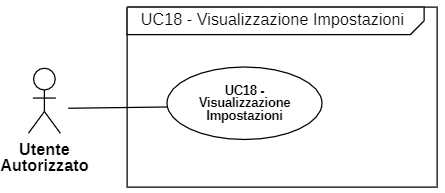
\includegraphics[scale=0.60]{images/UC14.png} 
		\caption{Descrizione grafica caso d'uso UC14}
	 \end{figure}

	\item \textbf{Attori}
	\begin{itemize} 
		\item \textit{Primari}: Utente autorizzato e non autenticato nella \glossario{Piattaforma Riunioni} esterna
		\item \textit{Secondari}: Piattaforma Riunioni esterna
	\end{itemize}
	\item \textbf{Descrizione}: L'utente vuole eseguire il login su \glossario{Piattaforma Riunioni} esterna.
	\item \textbf{Precondizione}: L'utente non ha un \glossario{access token} della piattaforma Riunioni necessario per inserire riunioni sull'app esterna.
	\item \textbf{Postcondizione}: L'utente riceve il link per effettuare il login ed ottenere l'\glossario{access token}.
	\item \textbf{Scenario principale}: \begin{enumerate}
		\item Utente deve fare il login (UC14.1) ed il bot fornisce il link per effettuare il login su \glossario{Piattaforma Riunioni} esterna; 
		\item Utente inserisce \glossario{access token} ricevuto dopo aver effettuato il login. (UC14.3)
	\end{enumerate}
\end{itemize}

\subsubsection{UC14.1 - Autenticazione su Piattaforma Riunioni esterna }
\begin{itemize}
	\item \textbf{Identificativo}: UC14.1
	\item \textbf{Nome}: Autenticazione su Piattaforma Riunioni esterna
	\item \textbf{Attori}
	\begin{itemize} 
		\item \textit{Primari}: Utente autorizzato
		\item \textit{Secondari}: Piattaforma Riunioni esterna
	\end{itemize}
	\item \textbf{Descrizione}: L'utente vuole eseguire il login su \glossario{Piattaforma Riunioni} esterna per poter creare riunioni.
	\item \textbf{Precondizione}: L'utente non ha eseguito il login su \glossario{Piattaforma Riunioni} esterna.
	\item \textbf{Postcondizione}: L'utente ha eseguito il login su \glossario{Piattaforma Riunioni} esterna.
	\item \textbf{Scenario principale}: \begin{enumerate}
		\item Utente esegue il login su \glossario{Piattaforma Riunioni} esterna; 
	\end{enumerate}
\end{itemize}

\subsubsection{UC14.2 - Errore Autenticazione su Piattaforma Riunioni esterna}
\begin{itemize}
	\item \textbf{Identificativo}: UC14.2
	\item \textbf{Nome}: Errore Autenticazione su Piattaforma Riunioni esterna
	\item \textbf{Attori}
	\begin{itemize} 
		\item \textit{Primari}: Utente autorizzato
		\item \textit{Secondari}: Piattaforma Riunioni esterna
	\end{itemize}
	\item \textbf{Descrizione}: L'utente vuole eseguire il login su \glossario{Piattaforma Riunioni} esterna ma incontra un errore.
	\item \textbf{Precondizione}: L'utente non ha eseguito il login su \glossario{Piattaforma Riunioni} esterna.
	\item \textbf{Postcondizione}: L'utente non riesce ad eseguire il login su \glossario{Piattaforma Riunioni} esterna ed il bot visualizza l'errore.
	\item \textbf{Scenario principale}: \begin{enumerate}
		\item Chatbot comunica : "Errore nella procedura di autenticazione". 
	\end{enumerate}
\end{itemize}

\subsubsection{UC14.3 - Inserimento \glossario{access token} per autenticazione }
\begin{itemize}
	\item \textbf{Identificativo}: UC14.3
	\item \textbf{Nome}: Inserimento \glossario{access token} per autenticazione
	\item \textbf{Attori}
	\begin{itemize} 
		\item \textit{Primari}: Utente autorizzato
		\item \textit{Secondari}: Nessuno
	\end{itemize}
	\item \textbf{Descrizione}: L'utente vuole eseguire il login su \glossario{Piattaforma Riunioni} esterna.
	\item \textbf{Precondizione}: L'utente ha ottenuto un \glossario{access token} della piattaforma Riunioni necessario per inserire riunioni su app esterna.
	\item \textbf{Postcondizione}: L'utente inserisce l'\glossario{access token} appena ricevuto.
	\item \textbf{Scenario principale}: \begin{enumerate}
		\item Utente inserisce l'\glossario{access token} ricevuto a seguito del login; 
	\end{enumerate}
\end{itemize}

\subsubsection{UC14.4 - Errore Inserimento access token }
\begin{itemize}
	\item \textbf{Identificativo}: UC14.4
	\item \textbf{Nome}: Errore Inserimento access token
	\item \textbf{Attori}
	\begin{itemize} 
		\item \textit{Primari}: Utente autorizzato
		\item \textit{Secondari}: Nessuno
	\end{itemize}
	\item \textbf{Descrizione}: L'utente vuole eseguire il login su \glossario{Piattaforma Riunioni} esterna ma incontra un errore nell'inserimento dell'access token.
	\item \textbf{Precondizione}: L'utente ha ottenuto un \glossario{access token} della piattaforma Riunioni necessario per inserire riunioni su app esterna.
	\item \textbf{Postcondizione}: L'utente inserisce l'\glossario{access token} della piattaforma Riunioni appena ricevuto ma viene notificato con un errore.
	\item \textbf{Scenario principale}: \begin{enumerate}
		\item Utente inserisce l'\glossario{access token} ricevuto a seguito del login; 
		\item Chatbot notifica Utente dell'impossibilità di compiere quest'azione.
	\end{enumerate}
\end{itemize}

\subsection{UC15 - Visualizzazione ore da consuntivare rimanenti }
\begin{itemize}
	\item \textbf{Identificativo}: UC15
	\item \textbf{Nome}: Visualizzazione ore da consuntivare rimanenti
	\item \textbf{Attori}
	\begin{itemize} 
		\item \textit{Primari}: Utente autorizzato
		\item \textit{Secondari}: Nessuno
	\end{itemize}
	\item \textbf{Descrizione}: L'utente visualizza le ore rimanenti da consuntivare nella giornata.
	\item \textbf{Precondizione}: L'utente ha consuntivato un'attività.
	\item \textbf{Postcondizione}: Il chatbot notifica il numero rimanente di ore da consuntivare nella giornata.
	\item \textbf{Scenario principale}: \begin{enumerate}
		\item Chatbot comunica: "Hai ancora X ore da consuntivare".
	\end{enumerate}
\end{itemize}
\subsubsection{UC15.1 - Visualizzazione elenco documenti Trovati}
\begin{itemize}
	\item \textbf{Identificativo}: UC15.1
	\item \textbf{Nome}: Visualizzazione elenco documenti Trovati
	\item \textbf{Attori}
	\begin{itemize} 
		\item \textit{Primari}: Utente autorizzato
		\item \textit{Secondari}: Nessuno
	\end{itemize}
	\item \textbf{Descrizione}: L'utente viene informato della ricerca dei documenti trovati.
	\item \textbf{Precondizione}: L'utente ha effettuato la ricerca con successo.
	\item \textbf{Postcondizione}: Il chatbot invia all'utente l'elenco dei documenti.
	\item \textbf{Scenario principale}: \begin{enumerate}
		\item Chatbot comunica: "Ho trovato questi documenti ..." seguito dall'elenco dei documenti trovati.
	\end{enumerate}
\end{itemize}

\subsection{UC16 - (teoricamente da cancellare) Visualizzazione elenco documenti Trovati }
\begin{itemize}
	\item \textbf{Identificativo}: UC16
	\item \textbf{Nome}: Visualizzazione elenco documenti Trovati
	\item \textbf{Attori}
	\begin{itemize} 
		\item \textit{Primari}: Utente autorizzato
		\item \textit{Secondari}: Nessuno
	\end{itemize}
	\item \textbf{Descrizione}: L'utente viene informato della ricerca dei documenti trovati.
	\item \textbf{Precondizione}: L'utente ha effettuato la ricerca con successo.
	\item \textbf{Postcondizione}: Il chatbot invia all'utente l'elenco dei documenti.
	\item \textbf{Scenario principale}: \begin{enumerate}
		\item Chatbot comunica: "Ho trovato questi documenti ..." seguito dall'elenco dei documenti trovati.
	\end{enumerate}
\end{itemize}

\subsection{UC17 - Visualizzazione Riunioni Giornaliere }
\begin{itemize}
	\item \textbf{Identificativo}: UC17
	\item \textbf{Nome}: Visualizzazione Riunioni Giornaliere
	\item \textbf{Attori}
	\begin{itemize} 
		\item \textit{Primari}: Utente autorizzato e autenticato nella \glossario{piattaforma riunioni}
		\item \textit{Secondari}: Non presenti
	\end{itemize}
	\item \textbf{Descrizione}: L'utente richiede di visualizzare le Riunioni del giorno.
	\item \textbf{Precondizione}: L'utente ha effettuato il login sia sull'app che sulla piattaforma esterna, e si trova nella chat.
	\item \textbf{Postcondizione}: Il chatbot restituisce la lista delle riunioni del giorno, con eventuali informazioni.
	\item \textbf{Scenario principale}:  \begin{enumerate}
		\item Utente invia un messaggio al chatbot : "Che riunioni ho oggi?";
		\item Chatbot restituisce la lista delle riunioni, con eventuali informazioni.
	\end{enumerate}
\end{itemize}

\subsection{UC18 - Visualizzazione Impostazioni}
\begin{itemize}
	\item \textbf{Identificativo}: UC18
	\item \textbf{Nome}: Visualizzazione Impostazioni
	\item \textbf{Attori}
	\begin{itemize} 
		\item \textit{Primari}: Utente autorizzato
		\item \textit{Secondari}: Non presenti
	\end{itemize}
	\item \textbf{Descrizione}: L'utente richiede la visualizzazione delle impostazioni.
	\item \textbf{Precondizione}: L'utente ha effettuato il login e si trova nella chat.
	\item \textbf{Postcondizione}: L'utente visualizza le impostazioni dell'applicazione.
	\item \textbf{Scenario principale}: \begin{enumerate}
		\item Utente interagisce con specifico pulsante per mostrare impostazioni;
		\item Utente visualizza le impostazioni.
	\end{enumerate}
\end{itemize}

\subsection{UC19 - Autenticazione su \glossario{Piattaforma Riunioni} esterna}
\begin{itemize}
	\item \textbf{Identificativo}: UC19
	\item \textbf{Nome}: Autenticazione su \glossario{Piattaforma Riunioni} esterna
	\item\textbf{Descrizione Grafica}: 
	\begin{center}
		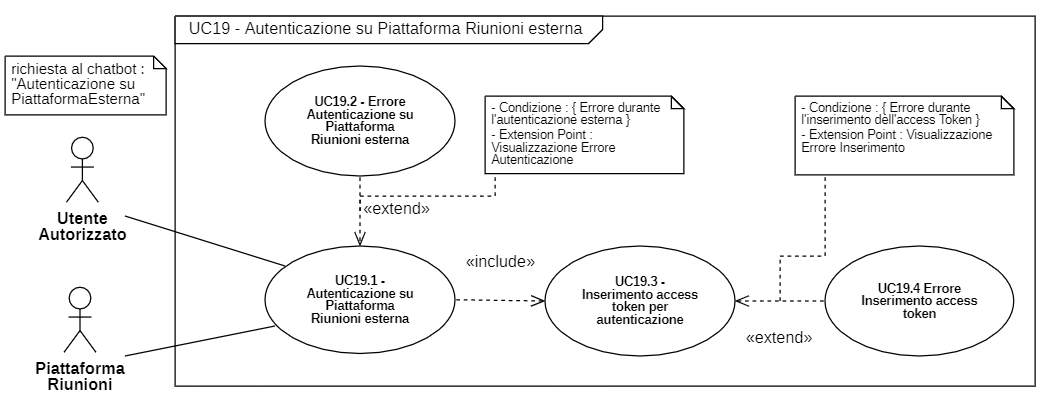
\includegraphics[scale=0.65]{images/UC19.png} 
	\end{center}

	\item \textbf{Attori}
	\begin{itemize} 
		\item \textit{Primari}: Utente autorizzato e non autenticato nella \glossario{Piattaforma Riunioni} esterna
		\item \textit{Secondari}: Piattaforma Riunioni esterna
	\end{itemize}
	\item \textbf{Descrizione}: L'utente vuole eseguire il login su \glossario{Piattaforma Riunioni} esterna.
	\item \textbf{Precondizione}: L'utente non ha un \glossario{access token} necessario per inserire riunioni sull'app esterna.
	\item \textbf{Postcondizione}: L'utente riceve il link per effettuare il login ed ottenere l'\glossario{access token}.
	\item \textbf{Scenario principale}: \begin{enumerate}
		\item Utente deve fare il login (UC19.1) ed il bot fornisce il link per effettuare il login su \glossario{Piattaforma Riunioni} esterna; 
		\item Utente inserisce \glossario{access token} ricevuto dopo aver effettuato il login. (UC19.3)
	\end{enumerate}
\end{itemize}

\subsubsection{UC19.1 - Autenticazione su Piattaforma Riunioni esterna }
\begin{itemize}
	\item \textbf{Identificativo}: UC19.1
	\item \textbf{Nome}: Autenticazione su Piattaforma Riunioni esterna
	\item \textbf{Attori}
	\begin{itemize} 
		\item \textit{Primari}: Utente autorizzato
		\item \textit{Secondari}: Piattaforma Riunioni esterna
	\end{itemize}
	\item \textbf{Descrizione}: L'utente vuole eseguire il login su \glossario{Piattaforma Riunioni} esterna per poter creare riunioni.
	\item \textbf{Precondizione}: L'utente non ha eseguito il login su \glossario{Piattaforma Riunioni} esterna.
	\item \textbf{Postcondizione}: L'utente ha eseguito il login su \glossario{Piattaforma Riunioni} esterna.
	\item \textbf{Scenario principale}: \begin{enumerate}
		\item Utente esegue il login su \glossario{Piattaforma Riunioni} esterna; 
	\end{enumerate}
\end{itemize}

\subsubsection{UC19.2 - Errore Autenticzione su Piattaforma Riunioni esterna}
\begin{itemize}
	\item \textbf{Identificativo}: UC19.2
	\item \textbf{Nome}: Errore Autenticzione su Piattaforma Riunioni esterna
	\item \textbf{Attori}
	\begin{itemize} 
		\item \textit{Primari}: Utente autorizzato
		\item \textit{Secondari}: Piattaforma Riunioni esterna
	\end{itemize}
	\item \textbf{Descrizione}: L'utente vuole eseguire il login su \glossario{Piattaforma Riunioni} esterna ma incontra un errore.
	\item \textbf{Precondizione}: L'utente non ha eseguito il login su \glossario{Piattaforma Riunioni} esterna.
	\item \textbf{Postcondizione}: L'utente non riesce ad eseguire il login su \glossario{Piattaforma Riunioni} esterna ed il bot visualizza l'errore.
	\item \textbf{Scenario principale}: \begin{enumerate}
		\item Chatbot comunica : "Errore nella procedura di autenticazione". 
	\end{enumerate}
\end{itemize}

\subsubsection{UC19.3 - Inserimento \glossario{access token} per autenticazione }
\begin{itemize}
	\item \textbf{Identificativo}: UC19.3
	\item \textbf{Nome}: Inserimento \glossario{access token} per autenticazione
	\item \textbf{Attori}
	\begin{itemize} 
		\item \textit{Primari}: Utente autorizzato
		\item \textit{Secondari}: Nessuno
	\end{itemize}
	\item \textbf{Descrizione}: L'utente vuole eseguire il login su \glossario{Piattaforma Riunioni} esterna.
	\item \textbf{Precondizione}: L'utente ha ottenuto un \glossario{access token} necessario per inserire riunioni su app esterna.
	\item \textbf{Postcondizione}: L'utente inserisce l'\glossario{access token} appena ricevuto.
	\item \textbf{Scenario principale}: \begin{enumerate}
		\item Utente inserisce l'\glossario{access token} ricevuto a seguito del login; 
	\end{enumerate}
\end{itemize}

\subsubsection{UC19.4 - Errore Inserimento access token }
\begin{itemize}
	\item \textbf{Identificativo}: UC19.4
	\item \textbf{Nome}: Errore Inserimento access token
	\item \textbf{Attori}
	\begin{itemize} 
		\item \textit{Primari}: Utente autorizzato
		\item \textit{Secondari}: Nessuno
	\end{itemize}
	\item \textbf{Descrizione}: L'utente vuole eseguire il login su \glossario{Piattaforma Riunioni} esterna ma incontra un errore nell'inserimento dell'access token.
	\item \textbf{Precondizione}: L'utente ha ottenuto un \glossario{access token} necessario per inserire riunioni su app esterna.
	\item \textbf{Postcondizione}: L'utente inserisce l'\glossario{access token} appena ricevuto ma viene notificato con un errore.
	\item \textbf{Scenario principale}: \begin{enumerate}
		\item Utente inserisce l'\glossario{access token} ricevuto a seguito del login; 
		\item Chatbot notifica Utente dell'impossibilità di compiere quest'azione.
	\end{enumerate}
\end{itemize}

\subsection{UC20 - Visualizzazione errore progetto non esistente}
\begin{itemize}
	\item \textbf{Identificativo}: UC20
	\item \textbf{Nome}: Visualizzazione errore progetto non esistente
	\item \textbf{Attori}
	\begin{itemize} 
		\item \textit{Primari}: Utente autorizzato
		\item \textit{Secondari}: Nessuno
	\end{itemize}
	\item \textbf{Descrizione}: L'utente inserisce i dati per inserimento dell'attività nel \glossario{SISTEMA EMT} aziendale.
	\item \textbf{Precondizione}: Utente ha inserito tutti i dati per effettuare l'inserimento.
	\item \textbf{Postcondizione}: Chatbot invia un messaggio di errore per progetto inesistente.
	\item \textbf{Scenario principale}: \begin{enumerate}
		\item Chatbot comunica l'errore: "Progetto Inesistente".
	\end{enumerate}
\end{itemize}

\subsection{UC21 - Visualizzazione errore progetto non esistente}
\begin{itemize}
	\item \textbf{Identificativo}: UC21
	\item \textbf{Nome}: Visualizzazione errore progetto non esistente
	\item \textbf{Attori}
	\begin{itemize} 
		\item \textit{Primari}: Utente autorizzato
		\item \textit{Secondari}: Non presenti
	\end{itemize}
	\item \textbf{Descrizione}: L'utente inserisce i dati per inserimento dell'\glossario{attività} nel \glossario{sistema EMT} aziendale.
	\item \textbf{Precondizione}: L'utente ha inserito correttamente tutti i dati per effettuare l'inserimento.
	\item \textbf{Postcondizione}: Il chatbot invia un messaggio di errore per progetto inesistente.
	\item \textbf{Scenario principale}: \begin{enumerate}
		\item Chatbot comunica l'errore: "Progetto Inesistente".
	\end{enumerate}
\end{itemize}


\newpage
\section{Requisiti}
Seguendo le Norme di Progetto ogni requisito è identificato da il suo codice, la sua descrizione e la fonte di provenienza.
\subsection{Requisiti Funzionali}
\begin{center}
\renewcommand{\arraystretch}{1.8} %aumento ampiezza righe
\begin{tabular}{ | m{8em} | m{18em} | m{12em} | }
\hline
Codice&Descrizione&Fonte\\
\hline
RO-F-1 & Il \glossario{ChatBot} deve poter riconoscere input testuale & Capitolato, UC1.1.1, UC2.1.1, UC3.1.1, UC4.1.1, UC5.1.1, UC5.2.1, UC5.3.1, UC5.4.1, UC6.1.1, UC6.2.1, UC7.1.1, UC7.2.1,  UC7.3.1, UC7.4.1, UC8.1.1, UC9.1.1, UC10.1.1, UC11.1.1 UC13.1.1\\
\hline
RO-F-2&Il \glossario{ChatBot} deve poter riconoscere input vocale&Capitolato, UC1.1.2, UC2.1.2, UC3.1.2, UC4.1.2, UC5.1.2, UC5.2.2, UC5.3.2, UC5.4.2, UC6.1.2, UC6.2.2, UC7.1.2, UC7.2.2,  UC7.3.2, UC7.4.2, UC8.1.2, UC9.1.2, UC10.1.2, UC11.1.2 UC13.1.2\\
\hline
RO-F-3&L’utente deve poter autenticarsi tramite un \glossario{token}&UC1\\
\hline
RO-F-4&Il programma deve poter riconoscere un \glossario{token} non valido&UC1\\
\hline
RO-F-5&Il programma deve poter far visualizzare un errore se il \glossario{token} non è valido&UC1.2\\
\hline
RO-F-6&L’utente non autenticato deve poter richiedere un \glossario{token} per autenticarsi&UC1.1\\
\hline
RD-F-7&Se l’utente ha più \glossario{token} a disposizione, può decidere quale usare.&Verbale Esterno\\
\hline
RO-F-8&L’utente deve poter effettuare la registrazione della propria presenza &UC2 \\
\hline
\end{tabular}
\end{center}
\begin{center}
\renewcommand{\arraystretch}{1.8} %aumento ampiezza righe
\begin{tabular}{ | m{8em} | m{18em} | m{12em} | }
\hline
RO-F-9&L’utente deve poter inserire la sede per la registrazione della presenza &UC2.1 \\
\hline
RO-F-10&Il \glossario{ChatBot} deve notificare l’utente se la sede per la registrazione non è valida &UC2.2 \\
\hline
RO-F-11&L’utente deve poter inserire un'\glossario{attività} all’interno del \glossario{sistema EMT} &UC3 \\
\hline
RO-F-12&L’utente deve poter inserire il tipo dell’\glossario{attività} &UC3.1 \\
\hline
RO-F-13&L’utente deve poter inserire le ore da consuntivare nell’\glossario{attività} &UC3.2 \\
\hline  
RO-F-14&L’utente deve poter inserire il progetto da consuntivare nell’\glossario{attività} &UC3.3 \\
\hline
RO-F-15&L’utente deve poter inserire il luogo in cui ha svolto l’\glossario{attività} &UC3.4 \\
\hline
RO-F-16&Il \glossario{ChatBot} deve notificare l'utente se l'\glossario{attività} è in un formato non valido &UC3.5 \\
\hline
RO-F-17&Il \glossario{ChatBot} deve notificare l'utente se le ore sono in un formato non valido &UC3.6 \\
\hline
RO-F-18&Il \glossario{ChatBot} deve notificare l'utente se il nome del progetto di un'\glossario{attività} è in un formato non valido &UC3.7 \\
\hline
RO-F-19&Il \glossario{ChatBot} deve notificare l'utente se il luogo relativo all’\glossario{attività} è in un formato non valido &UC3.8 \\
\hline
RD-F-20&L’utente deve poter aprire il cancello di un sede tramite \glossario{ChatBot} &UC4 \\
\hline
RO-F-21&L’utente deve poter inserire la sede in cui vuole aprire il candello &UC4.1 \\
\hline
RD-F-22&Il \glossario{ChatBot} deve notificare l'utente se la sede indicata non è valida &UC4.2 \\
\hline
RD-F-23&L’utente deve poter creare, tramite il \glossario{ChatBot}, una riunione su un'applicazione esterna &UC5 \\
\hline
\end{tabular}
\end{center}
\begin{center}
\renewcommand{\arraystretch}{1.8} %aumento ampiezza righe
\begin{tabular}{ | m{8em} | m{18em} | m{12em} | }
\hline
RD-F-24&L’utente deve poter inserire il nome della piattaforma esterna per la videoconferenza &UC5.1 \\
\hline
RD-F-25&L’utente deve poter inserire la data per la riunione &UC5.2 \\
\hline
RD-F-26&L’utente deve poter inserire l’ora per la riunione &UC5.3 \\
\hline
RD-F-27&L’utente deve poter inserire i partecipanti alla riunione &UC5.4 \\
\hline
RD-F-28&Il \glossario{ChatBot} deve notificare l’utente se la piattaforma inserita non è valida o non è supportata &UC5.5 \\
\hline
RD-F-29&Il \glossario{ChatBot} deve notificare l’utente se la data inserita non è valida o è indisponibile &UC5.6 \\
\hline
RD-F-30&Il \glossario{ChatBot} deve notificare l’utente se l’ora inserita non è valida o è indisponibile &UC5.7 \\
\hline
RD-F-31&Il \glossario{ChatBot} deve notificare l’utente se i partecipanti inseriti non sono corretti, chiedendo il reinserimento &UC5.8 \\
\hline
RD-F-32&L’utente deve poter chiedere di cercare un documento &UC6 \\
\hline
RD-F-33&L’utente deve poter inserire il nome del progetto per la ricerca del documento &UC6.1 \\
\hline
RD-F-34&L’utente deve poter inserire il nome del documento in cui vuole fare la ricerca &UC6.2 \\
\hline
RD-F-35&Il \glossario{ChatBot} deve notificare l’utente se l’inserimento del progetto non è corretto, chiedendo il reinserimento &UC6.3\\
\hline
RD-F-36&Il \glossario{ChatBot} deve notificare l’utente se il nome del documento inserito non è valido, chiedendo il reinserimento &UC6.4 \\
\hline
RD-F-37&L’utente deve poter inserire un \glossario{ticket} &UC7 \\
\hline
\end{tabular}
\end{center}
\begin{center}
\renewcommand{\arraystretch}{1.8} %aumento ampiezza righe
\begin{tabular}{ | m{8em} | m{18em} | m{12em} | }
\hline
RD-F-38&L’utente deve poter fornire l’oggetto per la creazione del \glossario{ticket} &UC7.1 \\
\hline
RD-F-39&L’utente deve poter inserire la descrizione per la creazione del \glossario{ticket} dopo aver fornito l’oggetto &UC7.2 \\
\hline
RD-F-40&L’utente deve poter inserire la priorità del \glossario{ticket} dopo aver comunicato lo status &UC7.3 \\
\hline
RD-F-41&Il \glossario{ChatBot} deve notificare l’utente se l’oggetto non è stato inserito in maniera idonea per la creazione del \glossario{ticket}  &UC7.4 \\
\hline
RD-F-42&Il \glossario{ChatBot} deve notificare l’utente se la priorità del \glossario{ticket} non è stato inserita in un formato valido &UC7.5 \\
\hline
RD-F-43&L’utente deve poter annullare un operazione precedentemente richiesto&UC8 \\
\hline
RD-F-44&Il \glossario{ChatBot} deve notificare l’utente se annullamento di un'operazione è con successo oppure impossibile&UC.2 \\
\hline
RD-F-45&L’utente deve poter richiedere lo stato di \glossario{Check-in}/Check-out&UC9.1 \\
\hline
RD-F-46&Il \glossario{ChatBot} deve notificare l’utente se la richiesta dello stato di \glossario{Check-in}/Check-out è impossibile&UC9.2 \\
\hline
RD-F-47&L’utente deve poter richiedere Ore Consuntivate&UC10 \\
\hline
RD-F-48&Il \glossario{ChatBot} deve notificare l’utente se la richiesta di visualizzazione ore consuntivate è impossibile &UC10.2 \\
\hline
RD-F-49&L’utente deve poter richiedere Ore Consuntivate&UC10 \\
\hline
RD-F-50&Il \glossario{ChatBot} deve notificare l’utente se la richiesta di visualizzazione di ore consuntivate è impossibile &UC10.2 \\
\hline
RD-F-51&L’utente deve poter richiedere Ore da Consuntivare rimanenti&UC11 \\
\hline
\end{tabular}
\end{center}
\begin{center}
\renewcommand{\arraystretch}{1.8} %aumento ampiezza righe
\begin{tabular}{ | m{8em} | m{18em} | m{12em} | }
\hline
RD-F-52&Il \glossario{ChatBot} deve notificare l’utente se la richiesta di visualizzazione di ore da consuntivare rimanenti è impossibile &UC11.2 \\
\hline
RD-F-53&L’utente deve poter visualizzare riunioni giornaliere&UC12 \\
\hline
RD-F-54&Il \glossario{ChatBot} deve notificare l’utente se la richiesta di visualizzazione riunioni giornaliere è impossibile &UC12.2 \\
\hline
RD-F-55&L’utente deve poter visualizzare le impostazioni&UC13\\
\hline
RD-F-56&L’utente deve poter autenticarsi su \glossario{Piattaforma Riunioni} esterna&UC14 \\
\hline
RD-F-57&Il \glossario{ChatBot} deve notificare l’utente l'autenticazione su \glossario{Piattaforma Riunioni esterna} è fallita &UC14.2 \\
\hline
RD-F-58&L’utente deve poter inserire il \glossario{access token} per autenticarsi su \glossario{Piattaforma Riunioni} esterna&UC14.3 \\
\hline
RD-F-59&Il \glossario{ChatBot} deve notificare l’utentese l'inserimento del \glossario{access roken} è fallita &UC14.4 \\
\hline
RD-F-60&Cifrare con il metodo \glossario{CBC-MAC} tutte le comunicazioni fra App e Server per garantire la validità delle informazioni&Capitolato\\
\hline
\end{tabular}
\end{center}
\newpage


\subsection{Requisiti di qualità}
\begin{center}
\renewcommand{\arraystretch}{1.8} %aumento ampiezza righe
\begin{tabular}{ | m{8em} | m{18em} | m{12em} | }
\hline
Codice&Descrizione&Fonte\\
\hline
RO-Q-1&Almeno l'80\% delle funzioni del programma deve essere testato e correlato dal report del test&Capitlato\\
\hline
RO-Q-2&Redarre documenti sulle scelte implementative e progettuali e relative motivazioni&Capitolato\\
\hline
RO-Q-3&Redarre documenti su problemi aperti e soluzioni possibili&Capitolato\\
\hline
RO-Q-4&Rispettare il piano di qualifica&Verbale interno\\
\hline
\end{tabular}
\end{center}

\subsection{Requisiti di vincolo}
\begin{center}
\renewcommand{\arraystretch}{1.8} %aumento ampiezza righe
\begin{tabular}{ | m{8em} | m{18em} | m{12em} | }
\hline
Codice&Descrizione&Fonte\\
\hline
RO-V-1&Utilizzare un applicazione mobile (per IOS 12 in poi o Android 4.1 in pois) che permette di utilizzare tutte le funzioni descritte dai requisiti funzionali&Capitolato\\
\hline
\end{tabular}
\end{center}

\newpage
\section{Tracciamento dei Requisiti}
Vengono qui raccolte e riassunte tutte le combinazioni requisito - fonte per motivi di praticità.
\subsection{Tracciamento filtrato per fonte}
\begin{center}
\renewcommand{\arraystretch}{1.8} %aumento ampiezza righe
\begin{tabular}{ |m{8em}|m{13em}| }
    \hline
    \textbf{Fonte} & \textbf{Requisito} \\
    \hline
    UC1         &   RO-F-3, RO-F-4 \\
    \hline
    UC1.1       &   RO-F-6 \\
    \hline
    UC1.1.1     &   RO-F-1 \\
    \hline
    UC1.1.2     &   RO-F-2 \\
    \hline
    UC1.2       &   RO-F-5 \\
    \hline
    UC2         &   RO-F-8, RO-F-9 \\
    \hline
    UC2.1.1     &   RO-F-1 \\
    \hline
    UC2.1.2     &   RO-F-2 \\
    \hline
    UC3         &   RO-F-10 \\
    \hline
    UC3.1       &   RO-F-11 \\
    \hline
    UC3.1.1     &   RO-F-1 \\
    \hline
    UC3.1.2     &   RO-F-2 \\
    \hline
    UC3.2       &   RO-F-12 \\
    \hline
    UC4         &   RO-F-13 \\
    \hline
    UC4.1       &   RO-F-14 \\
    \hline
    UC4.1.1     &   RO-F-1 \\
    \hline
    UC4.1.2     &   RO-F-2 \\
    \hline 
    UC4.2       &   RO-F-15 \\
    \hline
    UC4.3       &   RO-F-16 \\
    \hline
    UC4.4       &   RO-F-17 \\
    \hline
    \end{tabular}
    \newpage
    \begin{tabular}{ |m{8em}|m{13em}| }
    \hline
    UC4.5       &   RO-F-18 \\
    \hline
    UC4.6       &   RO-F-19 \\
    \hline
    UC4.7       &   RO-F-20 \\
    \hline
    UC4.8       &   RO-F-21 \\
    \hline
    UC5         &   RD-F-22 \\
    \hline
    UC5.1.1     &   RO-F-1 \\
    \hline
    UC5.1.2     &   RO-F-2 \\
    \hline
    UC5.2       &   RD-F-23 \\
    \hline
    UC6         &   RD-F-24 \\
    \hline
    UC6.1       &   RD-F-25 \\
    \hline
    UC6.1.1     &   RO-F-1 \\
    \hline
    UC6.1.2     &   RO-F-2 \\
    \hline
    UC6.2       &   RD-F-26 \\
    \hline
    UC6.2.1     &   RO-F-1 \\
    \hline
    UC6.2.2     &   RO-F-2 \\
    \hline
    UC6.3       &   RD-F-27 \\
    \hline
    UC6.3.1     &   RO-F-1 \\
    \hline
    UC6.3.2     &   RO-F-2 \\
    \hline
    UC6.4       &   RD-F-28 \\
    \hline
    UC6.4.1     &   RO-F-1 \\
    \hline
    UC6.4.2     &   RO-F-2 \\
    \hline
    UC6.5       &   RD-F-29 \\
    \hline
    UC6.6       &   RD-F-30 \\
    \hline
    UC6.7       &   RD-F-31 \\
    \hline
    UC6.8       &   RD-F-32 \\
    \hline
    UC7         &   RD-F-33 \\
    \hline
    \end{tabular}
    \newpage
    \begin{tabular}{ |m{8em}|m{13em}| }
    \hline
    UC7.1       &   RD-F-34 \\
    \hline
    UC7.1.1     &   RO-F-1 \\
    \hline
    UC7.1.2     &   RO-F-2 \\
    \hline
    UC7.2       &   RD-F-35 \\
    \hline
    UC7.2.1     &   RO-F-1 \\
    \hline
    UC7.2.2     &   RO-F-2 \\
    \hline
    UC7.3       &   RD-F-36 \\
    \hline
    UC7.4       &   RD-F-37 \\
    \hline
    UC8         &   RD-F-38 \\
    \hline
    UC8.1       &   RD-F-39 \\
    \hline
    UC8.1.1     &   RO-F-1 \\
    \hline
    UC8.1.2     &   RO-F-2 \\
    \hline
    UC8.2       &   RD-F-40 \\
    \hline
    UC8.2.1     &   RO-F-1 \\
    \hline
    UC8.2.2     &   RO-F-2 \\
    \hline
    UC8.3       &   RD-F-41 \\
    \hline
    UC8.3.1     &   RO-F-1 \\
    \hline
    UC8.3.2     &   RO-F-2 \\
    \hline
    UC8.4       &   RD-F-42 \\
    \hline
    UC8.4.1     &   RO-F-1 \\
    \hline
    UC8.4.2     &   RO-F-2 \\
    \hline
    UC8.5       &   RD-F-43 \\
    \hline
    UC8.6       &   RD-F-44 \\
    \hline
    UC8.7       &   RD-F-45 \\
    \hline
    \end{tabular}
    \newpage
    \begin{tabular}{ |m{8em}|m{13em}| }
    \hline
    UC9         &   RO-F-46 \\
    \hline
    UC10        &   RO-F-47 \\
    \hline
    UC11        &   RO-F-48, RO-F-49 \\
    \hline
    UC12        &   RO-F-50 \\
    \hline
    UC13        &   RO-F-51, RO-F-52 \\
    \hline
    UC14        &   RO-F-53 \\
    \hline
    UC15        &   RO-F-54 \\
    \hline
    UC16        &   RD-F-55 \\
    \hline
    UC17        &   RD-F-56 \\
    \hline
    UC18        &   RO-F-57 \\
    \hline
    UC19        &   RO-F-58 \\
    \hline
    UC19.1      &   RO-F-59 \\
    \hline
    UC20        &   RO-F-60 \\
    \hline
    UC21        &   RO-F-62 \\
    \hline
    Esterno     &   RD-F-7 \\
    \hline
    Interno     &   RO-Q-4 \\
    \hline
    Capitolato  &   RO-F-1, RO-F-2, RO-F-61, RO-Q-1, RO-Q-2, RO-Q-3, RO-V-1, RF-V-1 \\
    \hline
\end{tabular}
\end{center}
\subsection{Tracciamento filtrato per requisito}
\begin{center}
\renewcommand{\arraystretch}{1.8} %aumento ampiezza righe
\begin{tabular}{ |m{8em}|m{13em}| }
    \hline
    \textbf{Retuisito} & \textbf{Fonte} \\
    \hline
    RO-F-1  &   Capitolato, UC1.1.1, UC2.1.1, UC3.1.1, UC4.1.1, UC5.1.1, UC6.1.1, UC6.2.1, UC6.3.1, UC6.4.1, UC7.1.1, UC7.2.1, UC8.1.1, UC8.2.1, UC8.3.1, UC8.4.1 \\
    \hline
    RO-F-2  &   Capitolato, UC1.1.2, UC2.1.2, UC3.1.2, UC4.1.2, UC5.1.2, UC6.1.2, UC6.2.2, UC6.3.2, UC6.4.2, UC7.1.2, UC7.2.2, UC8.1.2, UC8.2.2, UC8.3.2, UC8.4.2 \\
    \hline
    RO-F-3  &   UC1 \\
    \hline
    RO-F-4  &   UC1 \\
    \hline
    RO-F-5  &   UC1.2 \\
    \hline
    RO-F-6  &   UC1.1 \\
    \hline
    RO-F-7  &   Esterno \\
    \hline
    RO-F-8  &   UC2 \\
    \hline
    RO-F-9  &   UC2 \\
    \hline
    RO-F-10  &  UC3 \\
    \hline
    RO-F-11  &  UC3.1 \\
    \hline
    RO-F-12  &  UC3.2, UC19 \\
    \hline
    RO-F-13  &  UC4 \\
    \hline
    RO-F-14  &  UC4.1 \\
    \hline
    RO-F-15  &  UC4.2 \\
    \hline
    RO-F-16  &  UC4.3 \\
    \hline
    RO-F-17  &  UC4.4 \\
    \hline
    RO-F-18  &  UC4.5 \\
    \hline
    \end{tabular}
    \newpage
    \begin{tabular}{ |m{8em}|m{13em}| }
    \hline
    RO-F-19  &  UC4.6 \\
    \hline
    RO-F-20  &  UC4.7, UC20 \\
    \hline
    RO-F-21  &  UC4.8 \\
    \hline
    RO-F-22  &  UC5 \\
    \hline
    RO-F-23  &  UC5.2 \\
    \hline
    RO-F-24  &  UC6 \\
    \hline
    RO-F-25  &  UC6.1 \\
    \hline
    RO-F-26  &  UC6.2 \\
    \hline
    RO-F-27  &  UC6.3 \\
    \hline
    RO-F-28  &  UC6.4 \\
    \hline
    RO-F-29  &  UC6.5 \\
    \hline
    RO-F-30  &  UC6.6 \\
    \hline
    RO-F-31  &  UC6.7 \\
    \hline
    RO-F-32  &  UC6.8 \\
    \hline
    RO-F-33  &  UC7 \\
    \hline
    RO-F-34  &  UC7.1 \\
    \hline
    RO-F-35  &  UC7.2 \\
    \hline
    RO-F-36  &  UC7.3 \\
    \hline
    RO-F-37  &  UC7.4 \\
    \hline
    RO-F-38  &  UC8 \\
    \hline
    RO-F-39  &  UC8.1 \\
    \hline
    RO-F-40  &  UC8.2 \\
    \hline
    RO-F-41  &  UC8.3 \\
    \hline
    RO-F-42  &  UC8.4 \\
    \hline
    RO-F-43  &  UC8.5 \\
    \hline
    \end{tabular}
    \newpage
    \begin{tabular}{ |m{8em}|m{13em}| }
    \hline
    RO-F-44  &  UC8.6 \\
    \hline
    RO-F-45  &  UC8.7 \\
    \hline
    RO-F-46  &  UC9 \\
    \hline
    RO-F-47  &  UC10 \\
    \hline
    RO-F-48  &  UC11 \\
    \hline
    RO-F-49  &  UC11 \\
    \hline
    RO-F-50  &  UC12 \\
    \hline
    RO-F-51  &  UC13 \\
    \hline
    RO-F-52  &  UC13 \\
    \hline
    RO-F-53  &  UC14 \\
    \hline
    RO-F-54  &  UC15 \\
    \hline
    RO-F-55  &  UC15.1 \\
    \hline
    RO-F-56  &  UC16 \\
    \hline
    RO-F-57  &  UC17 \\
    \hline
    RO-F-58  &  UC18 \\
    \hline
    RO-F-59  &  UC18.1 \\
    \hline
    RO-F-60  &  UC19 \\
    \hline
    RO-F-61  &  Capitolato \\
    \hline
    RO-F-62  &  UC20 \\
    \hline
    RO-Q-1  &  Capitolato \\
    \hline
    RO-Q-2  &  Capitolato \\
    \hline
    RO-Q-3  &  Capitolato \\
    \hline
    RO-Q-4  &  Interno \\
    \hline
    RO-V-1  &  Capitolato \\
    \hline
    RF-V-2  &  Capitolato \\
    \hline
\end{tabular}
\end{center}
\newpage

\end{document}